% ============================================================
%  main.tex  —  Overleaf master file (wmt-template compliant)
%  Paper: Multi-Objective Optimization of 2E-MD-MD-MP-CVRP-SPD
%         using INSGA3 (Triple-Initialization NSGA-III)
% ============================================================
\documentclass[11pt, a4paper]{article}

% ====== Preamble ======
\usepackage{wmt-template}
\usepackage[section]{placeins}   % keeps floats within their section
\usepackage{float}               % [H] exact placement
\usepackage{rotating}            % sidewaystable for wide comparison tables
\usepackage{tikz}
\usetikzlibrary{arrows.meta, fit, backgrounds, calc}

\addbibresource{references.bib}
\graphicspath{{./}{./figures/}}

\algnewcommand{\To}{\textbf{to }}
\algnewcommand{\Step}{\textbf{step }}

\studentname{Tse-An Wen}

% ── Custom math shorthands ────────────────────────────────────────
\newcommand{\KFE}{K_{\mathrm{FE}}}
\newcommand{\KSE}{K_{\mathrm{SE}}}
\newcommand{\NFE}{N_{\mathrm{FE}}}
\newcommand{\NSE}{N_{\mathrm{SE}}}
\newcommand{\QFE}{Q_{\mathrm{FE}}}
\newcommand{\QSE}{Q_{\mathrm{SE}}}
\newcommand{\cFE}{c_{\mathrm{FE}}}
\newcommand{\cSE}{c_{\mathrm{SE}}}
\newcommand{\eSE}{e_{\mathrm{SE}}}
\newcommand{\vSE}{v_{\mathrm{SE}}}

\newcommand{\CFE}{C_{\mathrm{FE}}}
\newcommand{\CSE}{C_{\mathrm{SE}}}
\newcommand{\CSat}{C_{\mathrm{sat}}}

\newcommand{\ESE}{E_{\mathrm{SE}}}

\widowpenalty=10000
\clubpenalty=10000

\algrenewcommand\algorithmicindent{1.2em}
\numberwithin{equation}{section}

\title{\textbf{Multi-Objective Optimization of the Two-Echelon Multi-Depot\\
Multi-Day Multi-Period Capacitated Vehicle Routing Problem\\
with Simultaneous Pickup and Delivery Using INSGA3}}

\author{Tse-An Wen}
\date{}

% ============================================================
\begin{document}
\maketitle
\thispagestyle{fancy}

% ─────────────────────────────────────────────────────────────
\begin{abstract}
This study addresses the two-echelon multi-depot multi-day multi-period
capacitated vehicle routing problem with simultaneous pickup and delivery
(2E-MD-MD-MP-CVRP-SPD, wherein the first ``MD'' denotes multi-depot and the
second ``MD'' denotes multi-day), a logistics optimization problem that
simultaneously minimizes total logistics cost, vehicle count, and carbon
emissions.  An Improved Non-dominated Sorting Genetic Algorithm~III (INSGA3)
is proposed, introducing a triple-method hybrid initialization strategy over
standard NSGA-III: Logistic Chaos Map initialization (diversity via chaotic
sequences, $r=3.9$), Spatial K-Medoids initialization (geographic
cluster-then-route), and Temporal-Spatial K-Medoids initialization (combined
geographic and time-window proximity).  Carbon emissions are quantified via
the MEET framework.  First-echelon routing is solved exactly by Gurobi MILP
after second-echelon routes are optimized by INSGA3.

Experiments on 20 benchmark instances (50- and 80-customer groups, 10
independent runs each) compare INSGA3 against standard NSGA-III, NSGA-II,
and MOVNS\@.  INSGA3 achieves an average cost of \$9{,}575.6, outperforming
NSGA-III by 9.3\%, NSGA-II by 10.0\%, and MOVNS by 25.8\%, with best
per-instance cost in 18 of 20 instances versus NSGA-III, 19 of 20 versus
NSGA-II, and all 20 instances versus MOVNS\@.  All four Pareto quality metrics (GD, IGD, HV, SC) consistently favor
INSGA3; specifically, GD\,=\,0.0214 vs.\ 0.0239 and IGD\,=\,0.0430
vs.\ 0.0476 against the best baseline, with INSGA3 also achieving superior
hypervolume (HV) and set coverage (SC) across all benchmark groups,
indicating that INSGA3's triple initialization
produces solutions more consistently proximate to the empirical Pareto
frontier.  The primary advantage of INSGA3 lies in the structured diversity
of the initial population, enabling the NSGA-III evolutionary loop to explore
higher-quality solution regions from the outset, demonstrating practical value
for large-scale green two-echelon logistics optimization.

\medskip
\noindent\textbf{Keywords:} Two-echelon vehicle routing problem;
Multi-objective optimization; NSGA-III; Chaos map initialization;
K-Medoids clustering; Temporal-spatial distance; Carbon emissions;
Green logistics
\end{abstract}

% ============================================================
\section{Introduction}
\label{sec:intro}
% ============================================================

This section establishes the motivation for studying the 2E-MD-MD-MP-CVRP-SPD,
defines the specific problem considered, identifies limitations in existing
solution approaches, and summarizes the contributions and organization of
the paper.

\subsection{Background and Motivation}

The global logistics industry has grown into one of the most critical pillars
of modern economies.  With the global logistics market projected to surpass
USD~12.6 trillion by~2027~\cite{grandview2020}, the pressure to deliver goods
efficiently, cost-effectively, and sustainably has reached unprecedented levels.  The
rise of e-commerce, the proliferation of urban distribution centers, and
increasingly dynamic customer demand patterns have collectively transformed
last-mile and two-echelon logistics into highly complex optimization challenges.

Vehicle Routing Problems (VRPs) constitute a fundamental class of combinatorial
optimization problems in logistics.  Among their extensions, the two-echelon
vehicle routing problem (2E-VRP) has attracted growing research interest as it
captures the two-tier distribution structure commonly observed in urban freight
systems: a first echelon connects central depots to intermediate facilities
(satellites), while a second echelon handles deliveries from satellites to end
customers.  Incorporating real-world constraints such as multiple depots,
multi-day planning horizons, multiple daily time periods, vehicle capacity
limits, and simultaneous pickup and delivery yields the
2E-MD-MD-MP-CVRP-SPD, a problem formulation that closely reflects operational
realities faced by modern logistics providers.

Beyond economic efficiency, environmental sustainability has become a central
concern for the logistics sector.  Transportation is responsible for
approximately 23\% of global CO$_2$ emissions~\cite{iea2022}, and regulatory
bodies worldwide are tightening emission standards.  Green logistics---the
integration of environmental objectives into route planning---has therefore
emerged as an important research direction.  In this study, carbon emissions
are quantified using the MEET framework~\cite{hickman1999}, and minimizing
carbon output is embedded as a third optimization objective alongside total
cost and vehicle count.

\subsection{Problem Overview}

The 2E-MD-MD-MP-CVRP-SPD considered in this study incorporates the following
real-world features:
\begin{enumerate}
  \item \textit{Two-echelon structure}: First-echelon vehicles transport goods
        from central depots to satellite facilities; second-echelon vehicles
        serve customers from satellites within prescribed time windows.
  \item \textit{Multi-depot}: Multiple central depots and multiple satellite
        locations are available, requiring joint optimization of depot-to-satellite
        and satellite-to-customer assignments.
  \item \textit{Multi-day and multi-period}: The planning horizon spans multiple
        days, and each day is divided into multiple service periods
        (e.g., morning and afternoon), with customer demand varying across both
        days and periods.
  \item \textit{Simultaneous pickup and delivery (SPD)}: Each second-echelon
        vehicle may collect returns from customers while delivering goods on the
        same route, demanding feasible load sequencing.
  \item \textit{Three-objective optimization}: The model simultaneously minimizes
        (i)~total logistics cost, (ii)~total number of vehicles deployed,
        and (iii)~total carbon emissions, forming a true multi-objective problem
        with non-trivial trade-offs.
\end{enumerate}

\subsection{Limitations of Existing Approaches}

Existing solution approaches for 2E-VRP variants predominantly rely on either
exact optimization (e.g., Gurobi-based MILP, branch-and-price) or classical
metaheuristics (e.g., NSGA-II, adaptive large neighborhood search~\cite{ropke2006}).  While
exact methods guarantee optimality, they scale poorly beyond small instances.
Classical evolutionary algorithms such as NSGA-II and standard NSGA-III often
suffer from:
\begin{enumerate}[label=(\roman*)]
  \item Poor initial solution quality due to random initialization;
  \item Insufficient diversity maintenance in later evolutionary stages;
  \item Weak local refinement capability at the chromosome level;
  \item Limited robustness across independent runs, producing high solution
        variance.
\end{enumerate}

\subsection{Proposed Approach and Contributions}

This study proposes INSGA3, which addresses the initialization limitation
through a triple-method hybrid strategy:
\begin{enumerate}
  \item \textbf{Logistic Chaos Map}: Generates each initial individual by
        ranking customers according to a chaotic sequence produced by the
        Logistic Map ($r=3.9$), ensuring high structural diversity across
        the initial population~\cite{may1976,ren2024}.
  \item \textbf{Spatial K-Medoids}: Partitions customers into $k$ geographic
        clusters via Partitioning Around Medoids (PAM), then builds each
        chromosome by routing within clusters via a nearest-neighbor
        heuristic~\cite{kaufman1990,wang2022collaborative}.
  \item \textbf{Temporal-Spatial K-Medoids}: Extends Spatial K-Medoids by
        replacing Euclidean distance with a normalized weighted combination
        of geographic and time-window proximity, capturing both spatial
        and scheduling structure~\cite{ren2024}.
\end{enumerate}

The main contributions are:
\begin{enumerate}
  \item A comprehensive three-objective 2E-MD-MD-MP-CVRP-SPD formulation
        integrating the MEET carbon emission model as a third optimization
        objective alongside total cost and vehicle count.
  \item The INSGA3 algorithm with a novel triple-method hybrid initialization
        strategy (Logistic Chaos Map, Spatial K-Medoids, Temporal-Spatial
        K-Medoids) that replaces random initialization in standard NSGA-III.
  \item A hybrid two-tier solution framework coupling INSGA3 (SE layer) with
        an exact Gurobi MILP solver (FE layer), enabling scalable optimization
        of the full two-echelon network.
  \item Empirical evaluation across 20 benchmark instances using Pareto quality
        metrics (GD, IGD, HV, SC), demonstrating superior Pareto front
        proximity and competitive cost reduction over NSGA-III and NSGA-II\@.
\end{enumerate}

\subsection{Paper Organization}

\Cref{sec:lit} reviews related literature.  \Cref{sec:model} presents the
mathematical model.  \Cref{sec:alg} describes INSGA3 and includes a worked
numerical example.  \Cref{sec:exp} reports computational experiments.
\Cref{sec:conc} concludes.

% ============================================================
\section{Literature Review}
\label{sec:lit}
% ============================================================

The following subsections survey the principal literature streams relevant to
the 2E-MD-MD-MP-CVRP-SPD: two-echelon routing and its structural extensions,
green VRP with carbon emission modeling, multi-objective evolutionary
algorithms applied to routing, and local search hybridization.  The section
closes by positioning the present work relative to the identified research gap.

\subsection{Two-Echelon VRP and Extensions}

The Vehicle Routing Problem, introduced by Dantzig and
Ramser~\cite{dantzig1959}, is among the most extensively studied problems in
operations research.  The Two-Echelon VRP (2E-VRP), formalized by
Perboli et al.~\cite{perboli2011} and Crainic et al.~\cite{crainic2011},
introduces intermediate satellite facilities between depots and customers.
Sluijk et al.~\cite{sluijk2023} provide a comprehensive survey systematically
categorizing 2E-VRP variants.

The SPD extension requires SE vehicles to collect returns from customers while
delivering goods on the same route.  Belgin et al.~\cite{belgin2018} proposed
one of the first exact models for 2E-CVRP-SPD\@.  Zhou
et al.~\cite{zhou2022spd} extended this to include time window constraints
and stochastic demand variants.

The multi-depot (MD) extension recognizes that real logistics networks feature
multiple warehouses.  Kancharla and Ramadurai~\cite{kancharla2019} formulated
MD-2E-VRP for urban freight, showing that coordinated satellite selection
significantly reduces total cost.

The multi-period dimension extends the planning horizon to multiple days.
Mourgaya and Vanderbeck~\cite{mourgaya2007} proposed a column generation
approach for multi-period VRP\@.  Wen et al.~\cite{wen2010} developed a
multi-period two-echelon model for city logistics.  Wang
et al.~\cite{wang2021} addressed multi-depot, multi-period collaborative
2E-VRP, and Wang et al.~\cite{wang2023} further extended this to a
location-routing formulation with pickup and delivery under vehicle sharing.
Each of these extensions addresses a specific structural dimension in isolation;
none jointly combines multi-depot, multi-day, multi-period, simultaneous pickup
and delivery, and three-objective optimization within a single two-echelon
routing framework.

\subsection{Green VRP and Carbon Emission Modeling}

Transportation accounts for approximately 23\% of global CO$_2$
emissions~\cite{iea2022}.  The MEET model~\cite{hickman1999} provides a
comprehensive multi-component emission estimation framework, decomposing
vehicle emissions into the base emission rate function $\varphi(v)$, the load
correction function $\psi(v)$, and the road slope correction $\gamma(v)$.
Li et al.~\cite{li2025} applied MEET to a multi-objective green VRP with time
windows, demonstrating that MEET-based objectives produce qualitatively
different Pareto frontiers compared to simple distance-based proxies.

Green 2E-VRP research has grown substantially.  Jepsen
et al.~\cite{jepsen2013} introduced a branch-and-cut exact method for the
symmetric two-echelon capacitated VRP\@.  Multi-objective green VRP
formulations show that Pareto-optimal trade-off frontiers between cost and
emissions are non-trivial and contain solutions qualitatively superior to
single-objective optima.
However, existing green VRP studies either adopt simplified distance-based
emission proxies rather than physics-grounded models such as MEET, or treat the
environmental objective in isolation rather than as part of a three-objective
Pareto framework; none integrates full MEET-based carbon modeling into a
two-echelon routing problem with simultaneous pickup and delivery.

\subsection{Multi-Objective Evolutionary Algorithms for VRP}

NSGA-II~\cite{deb2002nsga2} introduced fast non-dominated sorting and
crowding-distance-based selection, becoming the de facto reference MOEA for VRP
applications.  NSGA-III~\cite{deb2014nsga3} addresses its limitation in
three-or-more-objective problems by replacing crowding distance with structured
reference points uniformly distributed on a normalized hyperplane.

Standard NSGA-III exhibits weaknesses for VRP: random initialization produces
low-quality starting solutions, standard operators lack route-level insight,
and no explicit local-optima escape mechanism exists.  These weaknesses have
motivated improved NSGA-III variants incorporating transfer learning-based
initialization~\cite{improvedNSGA3transfer}, deep Q-learning guided operator
selection~\cite{dqlNSGA3}, and co-evolutionary strategies~\cite{coevNSGA3}.

Li et al.~\cite{li2025} proposed an improved NSGA-III (INSGA-III) for the
MOGVRPTW, incorporating nearest-neighbor initialization and selective 2-opt
on elite individuals, achieving significant cost reductions over NSGA-II and
NSGA-III on Solomon benchmarks.
The proposed INSGA3 in this study differs fundamentally: it applies a
\emph{triple-method} initialization combining chaotic diversity (Logistic
Chaos Map), geographic structure (Spatial K-Medoids), and joint
geographic-temporal structure (Temporal-Spatial K-Medoids), without embedded
local search, and couples the SE optimizer with exact FE MILP for the
substantially more complex 2E-MD-MD-MP-CVRP-SPD\@.
Despite these advances, no existing improved NSGA-III variant has been applied
to a multi-depot, multi-day, multi-period, SPD-constrained two-echelon problem,
nor has any prior work coupled a MOEA with an exact MILP solver for the
first-echelon tier.

\subsection{Initialization and Clustering Methods for VRP}

Initialization quality profoundly affects the trajectory and final quality of
evolutionary algorithms applied to VRP\@.  The nearest-neighbor heuristic
provides a deterministic starting sequence but lacks diversity across the
population~\cite{li2025}.  Chaos-based initialization using the Logistic
Map~\cite{may1976} has been applied to vehicle routing to generate structurally
diverse initial populations~\cite{ren2024}.  The Partitioning Around Medoids
(PAM) algorithm~\cite{kaufman1990} offers a robust alternative to k-means for
clustering when the cluster representative must be an actual data point,
making it suitable for constructing route structures from geographic
clusters~\cite{wang2022collaborative}.  Ren et al.~\cite{ren2024} further
extended spatial clustering with time-window information to form
temporal-spatial distance matrices that simultaneously capture geographic and
scheduling proximity.

The k-means clustering heuristic is widely used for customer-to-satellite
assignment in multi-satellite routing, providing a fast geometric partitioning
consistent with approaches reported for multi-satellite
2E-VRP~\cite{wang2021,wang2023}.
Local search operators including 2-opt~\cite{lin1965}, Or-opt~\cite{or1976},
and Variable Neighborhood Search~\cite{hansen2001} have demonstrated
effectiveness in post-initialization refinement, though they add computational
overhead per generation.  The proposed INSGA3 takes an alternative approach:
investing initialization effort through three complementary methods to provide
high-quality, diverse starting populations, without embedded local search.

\subsection{Research Gap and Positioning}

No existing study simultaneously addresses:
(1)~two-echelon structure with multiple depots and satellites; (2)~multi-day,
multi-period planning with period-dependent demand; (3)~SPD at the second
echelon; (4)~three competing objectives via MEET; and (5)~a MOEA with
triple-method hybrid initialization (Chaos Map, Spatial K-Medoids,
Temporal-Spatial K-Medoids) coupled with exact FE MILP\@.  The
2E-MD-MD-MP-CVRP-SPD and INSGA3 proposed in this study close this identified
gap.

% ============================================================
\section{Problem Statement and Mathematical Model}
\label{sec:model}
% ============================================================

This section formally defines the 2E-MD-MD-MP-CVRP-SPD, states the modeling
assumptions, introduces notation, and presents the complete three-objective
mathematical formulation including all first- and second-echelon constraints.

\subsection{Problem Statement}

The 2E-MD-MD-MP-CVRP-SPD is a multi-objective logistics optimization problem
defined over a two-level distribution network.  At the first echelon (FE),
large-capacity trucks transport consolidated freight from depots to satellites.
At the second echelon (SE), smaller vehicles depart from satellites to serve
customers simultaneously with deliveries and pickups.  The planning horizon
spans multiple days ($t\in T$), each divided into multiple service periods
($p\in P$), with customer demand varying across days and periods.

The system operates in three stages: (i)~k-means preprocessing clusters
customers to satellites; (ii)~INSGA3 determines SE vehicle routes for each
satellite-period block; (iii)~a Gurobi MILP solver optimizes FE routing given
the SE solution.  Three objectives are minimized simultaneously:
$f_1$~(total logistics cost), $f_2$~(total vehicle count), and
$f_3$~(total carbon emissions via MEET).

\subsection{Assumptions}

\begin{enumerate}
  \item All goods collected from customers are temporarily stored at the
        serving satellite before being returned to depots.
  \item Each customer has a soft service time window $[a_i^{t,p},\,b_i^{t,p}]$;
        early or late arrival incurs a penalty cost.
  \item The planning horizon covers multiple operational days, each subdivided
        into multiple periods; customers may appear at different locations on
        different days.
  \item Customer locations, delivery demands, and pickup quantities are known
        for each day and period.
  \item Each depot has sufficient stock capacity to supply all customer demands.
  \item Satellites are not subject to throughput capacity constraints.
  \item The total delivery load assigned to any SE vehicle route must not
        exceed $\QSE$ (departure capacity), and the total pickup load
        accumulated on the same route must not exceed $\QSE$ (return capacity).
        Dynamic load feasibility at intermediate stops is enforced by the
        load-tracking constraints presented in \cref{sec:model}.
  \item Each SE vehicle route must originate from and return to the same
        satellite.
  \item Delivery and pickup operations for each customer are performed
        simultaneously by the same vehicle on the same visit.
  \item SE vehicles cannot serve customers assigned to different satellites
        on a single route.
  \item All FE trucks are homogeneous with maximum load capacity $\QFE$;
        any truck may serve any depot-to-satellite arc.
  \item All SE vehicles are homogeneous with maximum load capacity $\QSE$;
        SE vehicles travel at fixed speed $\vSE = 50$~km/h.
  \item A single FE replenishment delivery on day~$t$ suffices to supply a
        satellite for all service periods of that day; the satellite is assumed
        to have sufficient intermediate storage capacity.  Consequently, the
        satellite-opening variable $z_s^{t,p}$ (period-level) and the FE
        routing variable $y_{ds}^{r,t}$ (day-level) operate on different time
        granularities: an open satellite in any period of day~$t$ requires at
        least one FE delivery on that day, but the FE delivery need not be
        period-specific.
\end{enumerate}

\subsection{Notation}

\paragraph{Sets and indices.}

\begin{tblr}{l l}
  $D,\,d$          & Set of depots; $d$ is the index \\
  $S,\,s$          & Set of satellites; $s$ is the index \\
  $C,\,i,j$        & Set of customers; $i,j$ are indices \\
  $T,\,t$          & Set of planning days; $t$ is the index \\
  $P,\,p$          & Set of service periods; $p$ is the index \\
  $\KFE,\,r$       & Set of FE trucks; $r$ is the index \\
  $\KSE,\,k$       & Set of SE vehicles; $k$ is the index \\
  $\NFE = D\cup S$ & Node set for FE routing \\
  $\NSE = S\cup C$ & Node set for SE routing \\
\end{tblr}

\paragraph{Parameters.}

\begin{tblr}{l l}
  $L_{ij}$              & Distance from node $i$ to node $j$ (km) \\
  $\vSE$                & SE vehicle speed (km/h) \\

  $TT_{ds}$             & Travel time from depot $d$ to satellite $s$ \\
  $DD_i^{t,p}$          & Delivery demand of customer $i$ on day $t$, period $p$ (kg) \\
  $DP_i^{t,p}$          & Pickup demand of customer $i$ on day $t$, period $p$ (kg) \\
  $DD_s^t$              & Total delivery demand at satellite $s$ on day $t$ (kg) \\
  $DP_s^t$              & Total pickup demand at satellite $s$ on day $t$ (kg) \\
  $\QSE$                & SE vehicle capacity (= 400 kg) \\
  $\QFE$                & FE vehicle capacity (= 4{,}000 kg) \\
  $\cSE$                & SE unit transportation cost (= 0.05 \$/km) \\
  $\cFE$                & FE unit transportation cost (= 0.2 \$/km) \\
  $F_r$                 & FE truck fixed deployment cost (= 80 \$) \\
  $F_k^{\mathrm{SE}}$   & SE vehicle fixed deployment cost (= 50 \$) \\
  $E_S$                 & Satellite deployment cost per day (\$) \\
  $\xi_e,\,\xi_l$       & Early/late arrival penalty rates (= 0.2 \$/min each) \\
  $a_d,\,b_d$           & Operating time window of depot $d$ \\
  $a_s^{t,p},b_s^{t,p}$ & Time window of satellite $s$ on day $t$, period $p$ \\
  $a_i^{t,p},b_i^{t,p}$ & Service time window of customer $i$ on day $t$, period $p$ \\
\end{tblr}

\paragraph{Decision variables.}

\begin{tblr}{l l}
  $x_{ij}^{k,s,t,p}\in\{0,1\}$           & 1 if SE vehicle $k$ travels arc $(i,j)$ at
                                             satellite $s$, day $t$, period $p$ \\
  $u_i^{k,s,t,p}\ge 0$                   & Cumulative delivery demand served up to customer $i$
                                             by SE vehicle $k$ (delivery MTZ variable) \\
  $v_i^{k,s,t,p}\ge 0$                   & Cumulative pickup collected up to customer $i$
                                             by SE vehicle $k$ (pickup MTZ variable) \\
  $A_i^{k,s,t,p}\ge 0$                   & Arrival time of SE vehicle $k$ at node $i$ \\
  $y_{ds}^{r,t}\in\{0,1\}$               & 1 if FE truck $r$ travels arc $(d,s)$ on day $t$ \\
  $f_{ds}^{r,t}\ge 0$                    & Freight volume on arc $(d,s)$ by truck $r$, day $t$ \\
  $ST_{dr}^t\ge 0$                       & Departure time of FE truck $r$ from depot $d$,
                                            day $t$ \\
  $VT_{sr}^t\ge 0$                       & Arrival time of FE truck $r$ at satellite $s$,
                                            day $t$ \\
  $z_s^{t,p}\in\{0,1\}$                  & 1 if satellite $s$ is open on day $t$, period $p$ \\
  $\omega_s^t\in\{0,1\}$                   & 1 if satellite $s$ is deployed on day $t$ \\
  $\delta_r^{\mathrm{FE},t}\in\{0,1\}$   & 1 if FE truck $r$ is deployed on day $t$ \\
  $\delta_k^{\mathrm{SE},t,p}\in\{0,1\}$ & 1 if SE vehicle $k$ is deployed on day $t$,
                                            period $p$ \\
\end{tblr}

\subsection{Mathematical Model}

The model comprises three objective functions minimizing cost, vehicle count,
and carbon emissions, together with two sets of routing constraints governing
the first and second echelons respectively.

\subsubsection{Objective Functions}

\paragraph{(f1) Total cost minimization.}
FE transportation cost $\CFE$ includes a distance-proportional term and a
per-truck fixed deployment cost:
\begin{equation}
  \CFE = \sum_{d\in D}\sum_{s\in S}\sum_{r\in\KFE}\sum_{t\in T}
           y_{ds}^{r,t}\,L_{ds}\,\cFE
         + \sum_{r\in\KFE}\sum_{t\in T}\delta_r^{\mathrm{FE},t}\,F_r
  \label{eq:CFE}
\end{equation}
where $\cFE = 0.2$ \$/km and $F_r = 80$ \$.  SE cost $\CSE$ combines
distance-proportional transport, a per-vehicle fixed deployment cost, and
soft time-window penalties:
\begin{equation}
  \CSE = \sum_{i,j\in\NSE}\sum_{k\in\KSE}\sum_{s\in S}\sum_{t\in T}\sum_{p\in P}
           x_{ij}^{k,s,t,p}\,L_{ij}\,\cSE
         + \sum_{k\in\KSE}\sum_{t\in T}\sum_{p\in P}\delta_k^{\mathrm{SE},t,p}\,F_k^{\mathrm{SE}}
         + \sum_{i\in C}\sum_{k\in\KSE}\sum_{s\in S}\sum_{t\in T}\sum_{p\in P}
           \Bigl[\xi_e\max\!\bigl(a_i^{t,p}-A_i^{k,s,t,p},0\bigr)
                +\xi_l\max\!\bigl(A_i^{k,s,t,p}-b_i^{t,p},0\bigr)\Bigr]
  \label{eq:CSE}
\end{equation}
where $\cSE=0.05$ \$/km; $F_k^{\mathrm{SE}}=50$ \$; $\xi_e=\xi_l=0.2$ \$/min;
morning vehicles depart satellite at $t=540$ min (09:00), afternoon at $t=720$ min (12:00).
The satellite deployment cost $E_S$ is charged once per satellite per day
it is deployed; the total satellite cost across all days is
\begin{equation}
  \CSat = E_S \sum_{t\in T}\sum_{s\in S} \omega_s^t
  \label{eq:CSat}
\end{equation}
where $\omega_s^t\in\{0,1\}$ indicates whether satellite $s$ is deployed on day $t$, and
$E_S = 500$ \$ in the benchmark experiments (\cref{tab:params}).
\begin{equation}
  \min\;f_1 = \CFE + \CSE + \CSat
  \label{eq:f1}
\end{equation}

\paragraph{(f2) Total vehicle count minimization.}
\begin{equation}
  \min\;f_2 = \sum_{t\in T}\sum_{p\in P}
    \Bigl(\sum_{r\in\KFE}\delta_r^{\mathrm{FE},t}
         +\sum_{k\in\KSE}\delta_k^{\mathrm{SE},t,p}\Bigr)
  \label{eq:f2}
\end{equation}

\paragraph{(f3) Total carbon emissions minimization.}
Carbon emissions are computed using the MEET model~\cite{hickman1999}.
For a 3.5-ton box truck (Table~A24 of~\cite{hickman1999}):
\begin{align}
  \varphi(v) &= 110 + 0.000375\,v^3 + \frac{8702}{v}
  \quad\text{(g CO}_2\text{/km)}
  \label{eq:phi} \\
  \psi(v)    &= 1.27 - 0.00235\,v - \frac{1.33}{v}
  \label{eq:psi}
\end{align}
The unit carbon emission is $\varphi(v)\cdot\psi(v)/1000$ (kg CO$_2$/km).
At the fixed SE speed $\vSE=50$ km/h:
\[
  \varphi(50)=330.915\;\text{g/km},\quad
  \psi(50)=1.1259,\quad
  \eSE=330.915\times1.1259/1000\approx0.3726\;\text{kg CO}_2\text{/km.}
\]
\begin{equation}
  \ESE = \sum_{i,j\in\NSE}\sum_{k\in\KSE}\sum_{s\in S}\sum_{t\in T}\sum_{p\in P}
           x_{ij}^{k,s,t,p}\,L_{ij}\,\eSE
  \label{eq:ESE}
\end{equation}
\begin{equation}
  \min\;f_3 = \ESE
  \label{eq:f3}
\end{equation}

\subsubsection{First-Echelon Constraints}

\begin{align}
  &\sum_{d\in D}\sum_{r\in\KFE}y_{ds}^{r,t} \ge z_s^{t,p},
  &&\forall\,s\in S,\,t\in T,\,p\in P
  \tag{C1}\label{c1}\\
  &\sum_{d\in D,s\in S}y_{ds}^{r,t}-\sum_{s\in S,d\in D}y_{sd}^{r,t}=0,
  &&\forall\,r\in\KFE,\,t\in T
  \tag{C2}\label{c2}\\
  &\sum_{d\in D,s\in S}y_{ds}^{r,t}(DD_s^t+DP_s^t)\le\QFE,
  &&\forall\,r\in\KFE,\,t\in T
  \tag{C3}\label{c3}\\
  &f_{ds}^{r,t}\ge 0,
  &&\forall\,d\in D,s\in S,r\in\KFE,t\in T
  \tag{C4a}\label{c4a}\\
  &\sum_{d\in D}f_{ds}^{r,t}-\sum_{d\in D}f_{sd}^{r,t}
    =\sum_{d\in D}y_{ds}^{r,t}\,(DD_s^t+DP_s^t),
  &&\forall\,s\in S,r\in\KFE,t\in T
  \tag{C4b}\label{c4b}\\
  &a_d\sum_{s\in S}y_{ds}^{r,t}\le ST_{dr}^t\le b_d\sum_{s\in S}y_{ds}^{r,t},
  &&\forall\,d\in D,r\in\KFE,t\in T
  \tag{C5}\label{c5}\\
  &ST_{dr}^t+TT_{ds}-M(1-y_{ds}^{r,t})\le VT_{sr}^t
    \le ST_{dr}^t+TT_{ds}+M(1-y_{ds}^{r,t}),
  &&\forall\,d,s,r\in\KFE,t
  \tag{C6}\label{c6}\\
  &y_{ds}^{r,t}\in\{0,1\},\quad
  f_{ds}^{r,t}\ge 0,\quad
  z_s^{t,p}\in\{0,1\},\quad
  \omega_s^t\in\{0,1\},
  &&\forall\,d,s,r,t,p
  \tag{C7}\label{c7}
\end{align}
\begin{align}
  &\omega_s^t \ge z_s^{t,p},
  &&\forall\,s\in S,\,t\in T,\,p\in P
  \tag{C8}\label{c8}
\end{align}

\subsubsection{Second-Echelon Constraints}

\begin{align}
  &\sum_{s\in S}\sum_{j\in\NSE}\sum_{k\in\KSE}x_{ij}^{k,s,t,p}=1,
  &&\forall\,i\in C,\,t\in T,\,p\in P
  \tag{C9}\label{c9}\\
  &\sum_{j\in\NSE}x_{ij}^{k,s,t,p}-\sum_{j\in\NSE}x_{ji}^{k,s,t,p}=0,
  &&\forall\,i\in\NSE,k\in\KSE,s,t,p
  \tag{C10}\label{c10}\\
  &\sum_{i\in C}\sum_{j\in\NSE}x_{ij}^{k,s,t,p}\,DD_i^{t,p}\le\QSE,
  &&\forall\,k\in\KSE,s\in S,t\in T,p\in P
  \tag{C11a}\label{c11a}\\
  &\sum_{i\in C}\sum_{j\in\NSE}x_{ij}^{k,s,t,p}\,DP_i^{t,p}\le\QSE,
  &&\forall\,k\in\KSE,s\in S,t\in T,p\in P
  \tag{C11b}\label{c11b}\\
  &\sum_{j\in C}x_{sj}^{k,s,t,p}=\sum_{j\in C}x_{js}^{k,s,t,p}\le 1,
  &&\forall\,k\in\KSE,s\in S,t\in T,p\in P
  \tag{C12}\label{c12}\\
  &u_i^{k,s,t,p}-u_j^{k,s,t,p}+\QSE\,x_{ij}^{k,s,t,p}\le\QSE-DD_j^{t,p},
  &&\forall\,i,j\in C,k,s,t,p
  \tag{C13a}\label{c13a}\\
  &DD_i^{t,p}\le u_i^{k,s,t,p}\le\QSE,
  &&\forall\,i\in C,k,s,t,p
  \tag{C13b}\label{c13b}\\
  &v_i^{k,s,t,p}-v_j^{k,s,t,p}+\QSE\,x_{ij}^{k,s,t,p}\le\QSE-DP_j^{t,p},
  &&\forall\,i,j\in C,k,s,t,p
  \tag{C13c}\label{c13c}\\
  &DP_i^{t,p}\le v_i^{k,s,t,p}\le\QSE,
  &&\forall\,i\in C,k,s,t,p
  \tag{C13d}\label{c13d}\\
  &A_j^{k,s,t,p}\ge A_i^{k,s,t,p}+\frac{L_{ij}}{\vSE}
    -M(1-x_{ij}^{k,s,t,p}),
  &&\forall\,i,j\in C,k,s,t,p
  \tag{C14}\label{c14}\\
  &a_s^{t,p}\sum_{j\in C}x_{sj}^{k,s,t,p}\le A_s^{k,s,t,p}
    \le b_s^{t,p}\sum_{j\in C}x_{sj}^{k,s,t,p},
  &&\forall\,k\in\KSE,s,t,p
  \tag{C15}\label{c15}\\
  &x_{ij}^{k,s,t,p}\in\{0,1\},\quad
  u_i^{k,s,t,p}\ge 0,\quad
  v_i^{k,s,t,p}\ge 0,\quad
  A_i^{k,s,t,p}\ge 0.
  \tag{C16}\label{c16}
\end{align}

\subsection{Model Summary}

The complete formulation is $\min\;\{f_1,f_2,f_3\}$ subject to
\cref{c1}--\cref{c7} (FE constraints), \cref{c8} (satellite deployment linking),
\cref{c9}--\cref{c16}
(SE constraints), with C11a--C11b replacing the single C11 for SPD capacity
and C13c--C13d providing pickup load tracking.  The problem is NP-hard (even
single-echelon CVRP is NP-hard); the INSGA3 + Gurobi decomposition
described in \cref{sec:alg} provides a practically scalable solution approach.

% ============================================================
\section{Proposed Algorithm: INSGA3}
\label{sec:alg}
% ============================================================

This section describes INSGA3 in detail, covering solution encoding,
the triple-method initialization strategy, the evolutionary operators,
and the complete algorithmic procedure including the Gurobi-based FE solver.

\subsection{Overview}

INSGA3 (Improved NSGA-III with Smart Initialisation) builds upon the
standard NSGA-III reference-point framework~\cite{deb2014nsga3} and
introduces a \emph{triple-method hybrid initialization} strategy that
replaces conventional random initialization with three structurally
distinct approaches.  The evolutionary loop follows the standard NSGA-III
procedure with OBX crossover and inversion mutation; no embedded local search
is applied.  FE routing is solved exactly by Gurobi MILP after SE routes are
finalized.  \Cref{fig:architecture} illustrates the overall data flow from
instance input to Pareto front output.

\begin{figure}[ht]
\centering
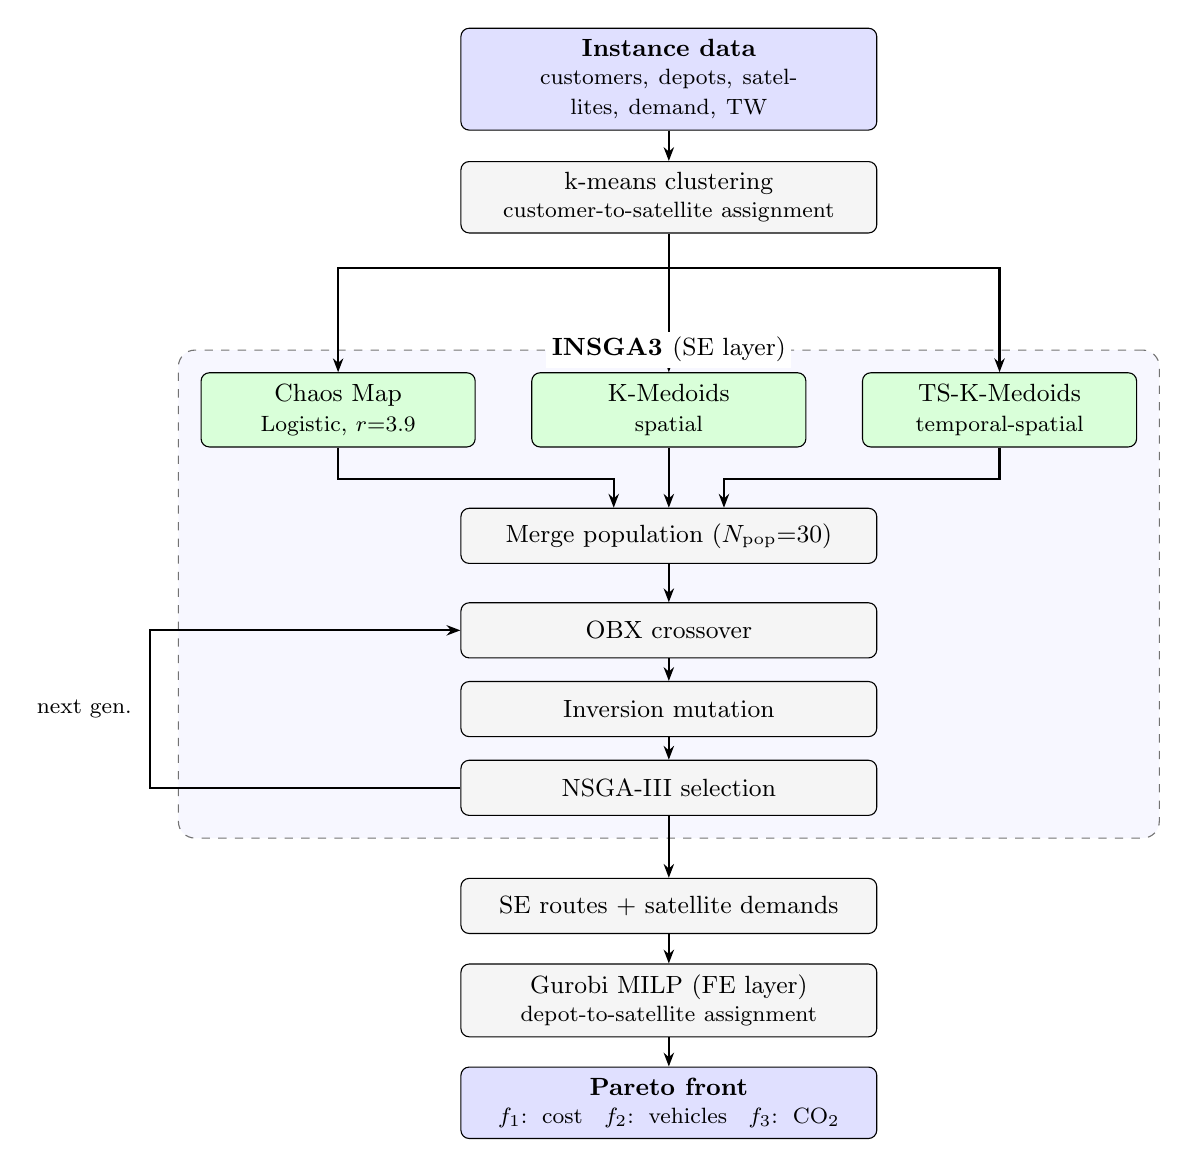
\begin{tikzpicture}[
  box/.style     = {draw, rounded corners=3pt, fill=gray!8,
                    text width=50mm, align=center, minimum height=7mm,
                    inner sep=4pt, font=\small},
  iobox/.style   = {draw, rounded corners=3pt, fill=blue!12,
                    text width=50mm, align=center, minimum height=7mm,
                    inner sep=4pt, font=\small\bfseries},
  initbox/.style = {draw, rounded corners=3pt, fill=green!15,
                    text width=32mm, align=center, minimum height=7mm,
                    inner sep=4pt, font=\small},
  arr/.style     = {-{Stealth[length=5pt]}, thick},
  looplabel/.style = {font=\footnotesize, midway, left=2pt},
]

\node[iobox]   (input)  at (0, 0.0)
  {Instance data\\[-1pt]
   {\normalfont\footnotesize customers, depots, satellites, demand, TW}};

\node[box]     (kmeans) at (0,-1.5)
  {k-means clustering\\[-1pt]
   {\footnotesize customer-to-satellite assignment}};

\node[initbox] (chaos)  at (-4.2,-4.2)
  {Chaos Map\\{\footnotesize Logistic, $r{=}3.9$}};
\node[initbox] (kmed)   at ( 0.0,-4.2)
  {K-Medoids\\{\footnotesize spatial}};
\node[initbox] (tskmed) at ( 4.2,-4.2)
  {TS-K-Medoids\\{\footnotesize temporal-spatial}};

\node[box]     (merge)  at (0,-5.8)
  {Merge population ($N_{\mathrm{pop}}{=}30$)};

\node[box]     (cross)  at (0,-7.0)  {OBX crossover};
\node[box]     (mut)    at (0,-8.0)  {Inversion mutation};
\node[box]     (sel)    at (0,-9.0)  {NSGA-III selection};

\node[box]     (sert)   at (0,-10.5)
  {SE routes + satellite demands};
\node[box]     (gurob)  at (0,-11.7)
  {Gurobi MILP (FE layer)\\[-1pt]
   {\footnotesize depot-to-satellite assignment}};
\node[iobox]   (out)    at (0,-13.0)
  {Pareto front\\[-1pt]
   {\normalfont\footnotesize $f_1$: cost \enspace $f_2$: vehicles \enspace
    $f_3$: CO$_2$}};

\begin{scope}[on background layer]
  \node[draw=black!55, dashed, rounded corners=6pt, fill=blue!3,
        inner sep=8pt,
        fit=(chaos)(kmed)(tskmed)(merge)(cross)(mut)(sel)] (insga3box) {};
\end{scope}
\draw[arr] (input)  -- (kmeans);
\draw[thick] (kmeans) -- ++(0,-0.90) coordinate (sp);
\draw[arr] (sp) -- ++(-4.2,0) -- (chaos.north);
\draw[arr] (sp) -- (kmed.north);
\draw[arr] (sp) -- ++( 4.2,0) -- (tskmed.north);
\draw[arr] (chaos.south)  -- ++(0,-0.4) -| ($(merge.north)+(-0.7,0)$);
\draw[arr] (kmed.south)   -- (merge.north);
\draw[arr] (tskmed.south) -- ++(0,-0.4) -| ($(merge.north)+(+0.7,0)$);
\draw[arr] (merge) -- (cross);
\draw[arr] (cross) -- (mut);
\draw[arr] (mut)   -- (sel);
\draw[arr] (sel)   -- (sert);
\draw[arr] (sert)  -- (gurob);
\draw[arr] (gurob) -- (out);

\draw[arr] (sel.west)
    -- (insga3box.west |- sel.west)
    -- ++(-0.35,0)
    -- ++(0,1.0) node[left=3pt, font=\footnotesize]{next gen.}
    -- ++(0,1.0)
    -- (insga3box.west |- cross.west)
    -- (cross.west);

\node[font=\small\bfseries, fill=white, inner sep=2pt] at (insga3box.north)
      {INSGA3 \textmd{(SE layer)}};

\end{tikzpicture}
\caption{System architecture and data flow of INSGA3 for
         2E-MD-MD-MP-CVRP-SPD\@.  The dashed border encloses the SE-layer
         evolutionary loop; the three green boxes show the triple-method
         initialization (executed once before the generational loop begins);
         the left arrow indicates the per-generation repeat.}
\label{fig:architecture}
\end{figure}

\subsection{Solution Encoding and Parameters}

Each chromosome is a permutation of customer IDs assigned to a given satellite
in a given time period.  For $|S|$ satellites and two daily periods,
$2|S|$ independent populations of size $N_{\mathrm{pop}}=30$ are maintained.
\Cref{tab:params} summarizes all algorithm parameters.

\begin{table}[ht]
\centering
\caption{INSGA3 Parameter Settings}
\label{tab:params}
\begin{tblr}{
    colspec = {l c},
}
\hline[0.08em]
Parameter & Value \\ \hline[0.05em]
Population size ($N_{\mathrm{pop}}$)              & 30 \\
Number of generations                             & 1{,}000 \\
Crossover probability ($cp$) --- Instances 1--10  & 0.65 \\
Crossover probability ($cp$) --- Instances 11--20 & 0.80 \\
Mutation probability ($mp$) --- Instances 1--10   & 0.60 \\
Mutation probability ($mp$) --- Instances 11--20  & 1.00 \\
Chaos parameter $r$                               & 3.9 \\
Temporal weight $\alpha$                          & 0.5 \\
SE vehicle capacity $\QSE$                        & 400 kg \\
SE vehicle speed $\vSE$                           & 50 km/h \\
SE vehicle fixed deployment cost $F_k^{\mathrm{SE}}$ & 50 \$ \\
FE vehicle capacity $\QFE$                        & 4{,}000 kg \\
Satellite deployment cost $E_S$                   & 500 \$ \\
Independent runs per instance                     & 10 \\ \hline[0.08em]
\end{tblr}
\end{table}

\subsection{Population Initialisation: Triple-Method Strategy}
\label{sec:init}

The $N_{\mathrm{pop}}=30$ individuals are generated by three complementary
methods, each contributing $\lfloor N_{\mathrm{pop}}/3 \rfloor = 10$
individuals; the remainder is allocated to Temporal-Spatial K-Medoids.
Each method exploits a different structural property of the problem.

\subsubsection{Method~1: Logistic Chaos Map}
\label{sec:init:chaos}

The Logistic Chaos Map~\cite{may1976,ren2024} generates diverse sequences
via the recurrence
\begin{equation}
  x_{k+1} = r\,x_k\,(1-x_k),\quad r=3.9,\quad x_0\sim\mathrm{Uniform}(0,1).
  \label{eq:chaos}
\end{equation}
For a customer set of size $n$, $n$ chaotic values $x_1,\ldots,x_n$ are
generated.  Customers are ranked by ascending chaotic value to obtain the
visit order.  Because the Logistic Map with $r=3.9$ exhibits fully chaotic
behavior~\cite{may1976}, different seeds $x_0$ produce structurally
uncorrelated permutations, maximising initial diversity.
(Chaotic values in \cref{sec:example} are truncated to four decimal places
for readability.)
\Cref{alg:chaos} describes the procedure.

\begin{algorithm}[ht]
\caption{Chaos Map initialization for one population slot}
\label{alg:chaos}
\begin{algorithmic}[1]
\Require Customer list $C=[c_1,\ldots,c_n]$, chaos parameter $r$
\Ensure Chromosome $\sigma$
\State $x \leftarrow \mathrm{Uniform}(0,1)$;\quad $\mathit{vals}\leftarrow[]$
       \Comment{Random seed; empty value list}
\For{$i=1$ \To $n$}
  \State $x \leftarrow r\cdot x\cdot(1-x)$;\quad
         $\mathit{vals}.\mathrm{append}(x)$
         \Comment{Logistic map iterate; record chaotic value}
\EndFor
\State $\sigma \leftarrow$ sort $C$ by ascending $\mathit{vals}$
       \Comment{Rank ascending $\Rightarrow$ visit order}
\State \Return $\sigma$
\end{algorithmic}
\end{algorithm}

\subsubsection{Method~2: Spatial K-Medoids}
\label{sec:init:kmed}

Spatial K-Medoids~\cite{kaufman1990,park2009,wang2022collaborative} partitions
customers into $k$ geographic clusters and routes each cluster via a
nearest-neighbour (NN) tour.  The number of clusters is
\begin{equation}
  k = \left\lceil\frac{\sum_{i\in C}(DD_i^{t,p}+DP_i^{t,p})}{\QSE}\right\rceil,
  \label{eq:kval}
\end{equation}
where $k$ is computed independently per satellite, day $t$, and period $p$,
ensuring each cluster can be served by a single SE vehicle.
The Partitioning Around Medoids (PAM) algorithm~\cite{kaufman1990} iterates
between assignment (each customer to the nearest medoid by Euclidean distance)
and medoid update (select the member minimising within-cluster total distance)
until convergence.  Within each cluster, customers are ordered by a
nearest-neighbour heuristic; clusters are sequenced by centroid distance
from the satellite with a random rotational offset.  \Cref{alg:kmed}
summarizes the procedure.

\begin{algorithm}[ht]
\caption{Spatial K-Medoids initialization for one population slot}
\label{alg:kmed}
\begin{algorithmic}[1]
\Require Customer list $C$, coordinate lookup \textit{coord},
         capacity $\QSE$, satellite coordinates
\Ensure Chromosome $\sigma$
\State $k \leftarrow \lceil\text{total demand}/\QSE\rceil$
       \Comment{Minimum vehicles required to cover demand}
\State $\mathit{medoids}\leftarrow\mathrm{random\_sample}(C,k)$
       \Comment{Random initial medoids}
\Repeat
  \State Assign each $c\in C$ to nearest medoid (Euclidean)
         \Comment{PAM assignment step}
  \State Update each medoid to member minimising within-cluster sum distance
         \Comment{PAM update step}
\Until{medoids unchanged} \Comment{PAM convergence}
\State Order customers within each cluster by NN heuristic
       \Comment{Intra-cluster route}
\State Sort clusters by centroid distance from satellite; apply random rotation
       \Comment{Inter-cluster order with diversity}
\State $\sigma\leftarrow$ concatenate ordered clusters
       \Comment{Assemble full chromosome}
\State \Return $\sigma$
\end{algorithmic}
\end{algorithm}

\subsubsection{Method~3: Temporal-Spatial K-Medoids}
\label{sec:init:tskmed}

Temporal-Spatial K-Medoids~\cite{ren2024} extends Method~2 by replacing the
purely geographic distance with a weighted combination of normalised spatial
and temporal proximity.  The combined distance matrix is
\begin{equation}
  D_{ij} = \alpha\,\bar{d}^{\mathrm{sp}}_{ij}
          +(1-\alpha)\,\bar{d}^{\mathrm{tm}}_{ij},\quad\alpha=0.5,
  \label{eq:ts_dist}
\end{equation}
where $\bar{d}^{\mathrm{sp}}_{ij}$ is the Haversine distance normalised by
the maximum pairwise spatial distance, and
$\bar{d}^{\mathrm{tm}}_{ij}=|m_i-m_j|/\max_{p,q}|m_p-m_q|$ with
$m_i=(a_i+b_i)/2$ the midpoint of customer $i$'s service time
window~\cite{ren2024}.  PAM clustering and within-cluster NN routing then
follow Method~2 (\cref{alg:kmed}) with $D_{ij}$ replacing Euclidean distance.

\subsection{Crossover: Order-Based Crossover (OBX)}

OBX selects a random contiguous segment $[a,b]$ from parent $p_1$, copies it
to offspring $c_1$ at the same positions, then fills remaining positions with
customers from $p_2$ in the order they appear, skipping already-placed
customers.  Offspring $c_2$ is generated symmetrically.

\subsection{Mutation Operator}

An inversion mutation~\cite{larranaga1999} is applied: a random sub-sequence
$[i,j]$ of the chromosome is reversed.  This produces route-level
restructuring while preserving chromosome feasibility.

\subsection{Selection: NSGA-III Reference-Point Framework}

The combined parent--offspring pool is reduced to $N_{\mathrm{pop}}$ using
standard NSGA-III~\cite{deb2014nsga3}: (1)~non-dominated sorting partitions
individuals into fronts $F_1,F_2,\ldots$; (2)~fronts are admitted until the
population would exceed $N_{\mathrm{pop}}$; (3)~reference points on the
normalised hyperplane govern niching selection in the critical last front.

\subsection{Complete Algorithm}

\Cref{alg:insga3} presents the complete INSGA3 procedure.

\begin{algorithm}[ht]
\caption{INSGA3 for 2E-MD-MD-MP-CVRP-SPD}
\label{alg:insga3}
\begin{algorithmic}[1]
\Require Instance data, parameters ($N_{\mathrm{pop}},cp,mp,r,\alpha,
         \mathrm{num\_gen}$)
\Ensure Best SE routes per satellite-period; FE cost
\State Cluster customers to satellites via k-means
       \Comment{Geographic pre-partitioning}
\State Partition customers into morning / afternoon periods
       \Comment{Time-period assignment}
\For{each satellite $s$ and period $p$}
  \State $\mathit{slots}\leftarrow\lfloor N_{\mathrm{pop}}/3\rfloor$
         \Comment{Equal slots per method}
  \State $P_1\leftarrow\mathrm{ChaosMap}(\mathrm{cust}_{s,p},\mathit{slots},r)$
         \Comment{Diversity via chaotic sequences; see \cref{alg:chaos}}
  \State $P_2\leftarrow\mathrm{KMedoids}(\mathrm{cust}_{s,p},\mathit{slots},\QSE)$
         \Comment{Geographic cluster seeding; see \cref{alg:kmed}}
  \State $P_3\leftarrow\mathrm{TSKMedoids}(\mathrm{cust}_{s,p},
         N_{\mathrm{pop}}-2\cdot\mathit{slots},\QSE,\alpha)$
         \Comment{Time-window-aware seeding; remainder slots}
  \State $P_{s,p}\leftarrow\mathrm{Merge}(P_1,P_2,P_3)$
         \Comment{Triple-method initial population}
\EndFor
\For{$\mathrm{gen}=1$ \To $\mathrm{num\_gen}$}
  \For{each population $P_{s,p}$}
    \If{$\mathrm{rand}()<cp$}
      \State $O\leftarrow\mathrm{OBX}(P_{s,p})$
             \Comment{Order-based crossover offspring}
    \Else
      \State $O\leftarrow\emptyset$
    \EndIf
    \State $O\leftarrow O\cup\mathrm{Mutate}(P_{s,p},mp)$
           \Comment{Inversion mutation}
    \State $P_{s,p}\leftarrow\mathrm{NSGA3\_Select}(P_{s,p}\cup O,N_{\mathrm{pop}})$
           \Comment{Non-dominated sort + reference-point niching}
  \EndFor
\EndFor
\State Extract best solution from each $P_{s,p}$
       \Comment{Retrieve SE routes from Pareto front for FE input}
\State Compute satellite demands from SE routes
       \Comment{Aggregate per-satellite delivery/pickup}
\State $\mathrm{FE\_cost}\leftarrow
       \mathrm{Gurobi\_MILP}(\mathrm{depots},\mathrm{satellites},\mathrm{demands})$
       \Comment{Exact first-echelon MILP}
\State \Return SE routes, FE cost
\end{algorithmic}
\end{algorithm}

\subsection{Complexity Analysis}
\label{sec:complexity}

Let $n$ denote the number of customers assigned to a single satellite-period
block, $N_{\mathrm{pop}}$ the population size, $G$ the number of generations,
$|S|$ the number of satellites, and $|P|=2$ the number of daily service
periods.

\paragraph{Time complexity.}
The dominant per-generation cost for each satellite-period population is
summarized in \cref{tab:complexity}.

\begin{table}[ht]
\centering
\caption{Per-component time complexity of INSGA3}
\label{tab:complexity}
\begin{tblr}{l l l}
\hline[0.08em]
Component & Complexity & Remark \\ \hline[0.05em]
Chaos Map init (once)      & $O(N_{\mathrm{pop}}\,n\log n)$ & Sort by chaotic values \\
Spatial K-Medoids (once)   & $O(N_{\mathrm{pop}}\,n^2)$     & PAM iterations \\
TS-K-Medoids (once)        & $O(N_{\mathrm{pop}}\,n^2)$     & Distance matrix + PAM \\
OBX crossover              & $O(N_{\mathrm{pop}}\,n)$        & Linear scan per offspring \\
Inversion mutation         & $O(N_{\mathrm{pop}}\,n)$        & Single-pass reversal \\
NSGA-III selection         & $O(N_{\mathrm{pop}}^2)$         & Fast non-dominated sort, 3 obj. \\
\hline[0.08em]
\end{tblr}
\end{table}

K-Medoids initialization dominates with $O(N_{\mathrm{pop}}\,n^2)$ but is
executed only once.  The overall SE-layer time complexity is
\begin{equation}
  O\!\bigl(|S|\cdot|P|\cdot N_{\mathrm{pop}}\cdot n^2\bigr)
  +O\!\bigl(G\cdot|S|\cdot|P|\cdot N_{\mathrm{pop}}\cdot n\bigr),
  \label{eq:time}
\end{equation}
where the first term is the one-time initialization cost and the second term
is the generational loop cost.  With $G=1{,}000$, $N_{\mathrm{pop}}=30$,
$|P|=2$, and $n\le 40$ customers per block, the generational loop operates at
$O(n)$ per individual per generation, achieving an average runtime of
71.4\,s per instance (maximum 110.7\,s; see \cref{tab:detail}).

The first-echelon Gurobi MILP is called once per algorithm run.  The FE
subproblem is compact ($|D|\times|S|$ binary arc variables per truck per day)
and solved rapidly by the branch-and-bound solver on these instances.

\paragraph{Space complexity.}
Each satellite-period population stores $N_{\mathrm{pop}}$ chromosomes of
length $n$ and fitness vectors of dimension~3.  The total space across all
blocks is
\begin{equation}
  O\!\bigl(|S|\cdot|P|\cdot N_{\mathrm{pop}}\cdot n\bigr).
  \label{eq:space}
\end{equation}
No additional data structures grow with $G$; memory consumption is independent
of the number of generations.

\subsection{Illustrative Numerical Example}
\label{sec:example}

To concretely illustrate how INSGA3 operates, this subsection traces each
algorithmic step through a small synthetic instance with one depot~$D$,
two satellites ($S_1$, $S_2$), and six customers ($C_1$--$C_6$) over a
single day and period.  \Cref{fig:illustrative_nodes} shows the node layout; $\QSE=20$ and $\QFE=30$ units.

\begin{figure}[ht]
\centering
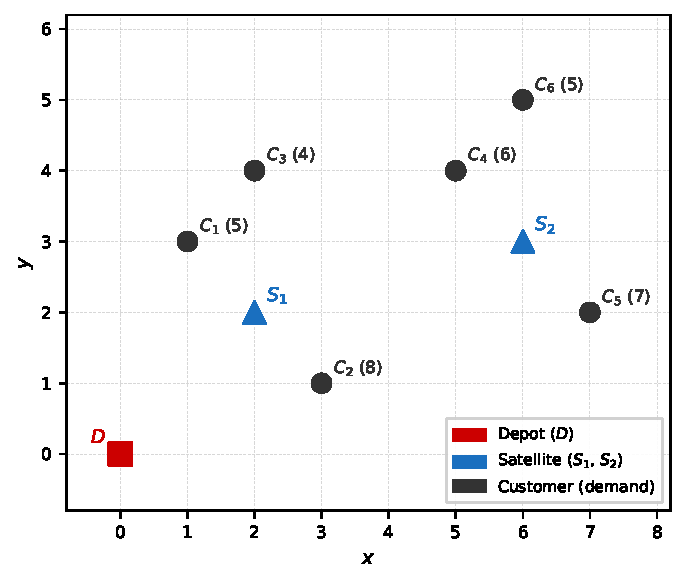
\includegraphics[width=0.55\linewidth]{illustrative_instance.pdf}
\caption{Node coordinates and demands for the illustrative instance.
         Numbers in parentheses denote customer demand.}
\label{fig:illustrative_nodes}
\end{figure}

\paragraph{Step 1 --- Spatial K-Medoids Clustering.}
Spatial K-Medoids ($k{=}2$) partitions customers by Euclidean proximity via
PAM\@.  \Cref{tab:illustrative_kmeans} shows the resulting assignment; both clusters
satisfy $\QSE=20$.  The remainder focuses on the $S_1$ sub-population
($n=3$ customers).

\begin{table}[ht]
\centering
\caption{K-Medoids customer-to-satellite assignment}
\label{tab:illustrative_kmeans}
\begin{tblr}{c c c}
\hline[0.08em]
Satellite & Customers assigned & Total demand \\ \hline[0.05em]
$S_1$ & $C_1,\,C_2,\,C_3$ & 17 \\
$S_2$ & $C_4,\,C_5,\,C_6$ & 18 \\
\hline[0.08em]
\end{tblr}
\end{table}

\paragraph{Step 2 --- Triple Initialization.}
Three chromosomes seed the $S_1$ sub-population via the three initialization
methods: the Chaos Map ($r=3.9$, $x_0=0.40$) ranks customers by ascending
chaotic value to yield $x_1=[C_2,\,C_3,\,C_1]$; Spatial K-Medoids orders
customers by medoid-proximity to yield $x_2=[C_1,\,C_2,\,C_3]$;
Temporal-Spatial K-Medoids incorporates time-window proximity to yield
$x_3=[C_3,\,C_1,\,C_2]$.

\paragraph{Step 3 --- OBX Crossover.}
OBX fixes gene~$C_3$ (selected from $x_2$ at position~3), then fills the
remaining positions with $x_1$'s genes in their original relative order,
skipping~$C_3$.  \Cref{fig:illustrative_obx} traces each step; the resulting
offspring is $o_1=[C_2,\,C_1,\,C_3]$.

\begin{figure}[ht]
\centering
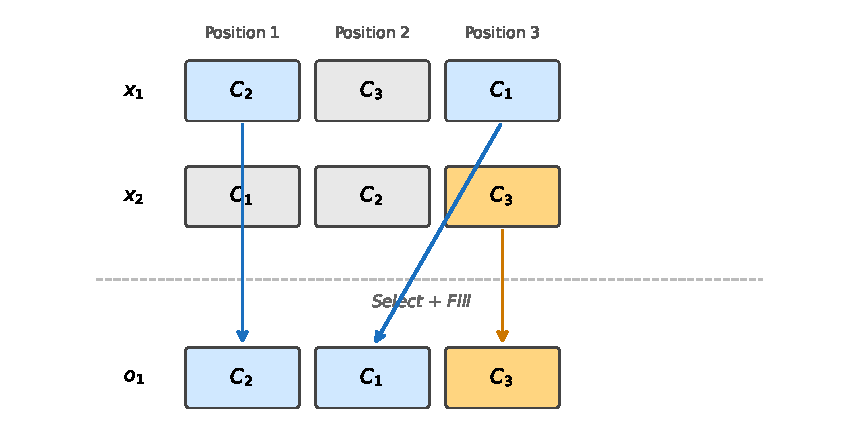
\includegraphics[width=0.65\linewidth]{obx_crossover.pdf}
\caption{OBX crossover: parent chromosomes, selected gene, and offspring.}
\label{fig:illustrative_obx}
\end{figure}

\paragraph{Step 4 --- Inversion Mutation.}
Given $x_3=[C_3,C_1,C_2]$, positions $\{1,2\}$ are randomly selected;
reversing the sub-sequence $[C_3,C_1]$ yields the mutant $m=[C_1,C_3,C_2]$.

\paragraph{Step 5 --- NSGA-III Selection.}
After evaluating all offspring on the three objectives ($f_1$: total cost,
$f_2$: number of vehicles, $f_3$: CO$_2$ emissions), fast non-dominated
sorting assigns each solution to a Pareto front.  \Cref{tab:illustrative_fronts}
illustrates a six-solution population.  Front~I contains $x_1$, $x_2$,
and $x_3$: none dominates another because each is better on at least one
objective.  NSGA-III selects all of Front~I first, then applies
reference-point niching among Front~II candidates for remaining slots,
repeating for $G$ generations before passing the aggregated Pareto front
to the Gurobi MILP for first-echelon routing.

\begin{table}[ht]
\centering
\caption{Non-dominated front assignment for the illustrative population}
\label{tab:illustrative_fronts}
\begin{tblr}{c r r r c}
\hline[0.08em]
Solution & $f_1$ (cost) & $f_2$ (NV) & $f_3$ (CO$_2$, kg) & Front \\ \hline[0.05em]
$x_1$ & 145 & 2 & 12.1 & I   \\
$x_2$ & 158 & 1 & 11.5 & I   \\
$x_3$ & 162 & 2 & 10.8 & I   \\
$x_4$ & 170 & 2 & 11.9 & II  \\
$x_5$ & 155 & 3 & 14.2 & II  \\
$x_6$ & 175 & 2 & 13.0 & III \\
\hline[0.08em]
\end{tblr}
\end{table}

\begin{figure}[ht]
\centering
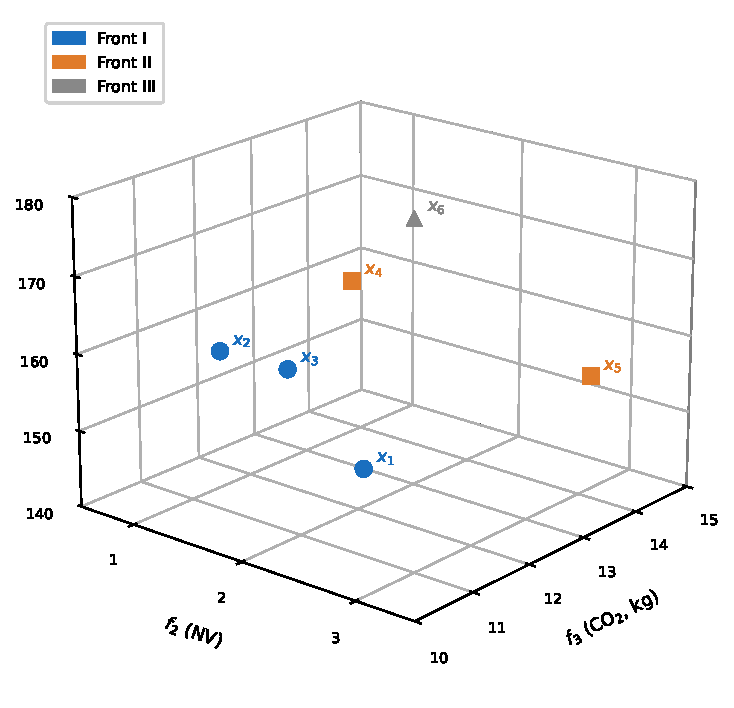
\includegraphics[width=0.60\linewidth]{illustrative_fronts_draft.pdf}
\caption{3D Pareto front visualization of the illustrative population}
\label{fig:illustrative_fronts}
\end{figure}

% ============================================================
\section{Computational Experiments}
\label{sec:exp}
% ============================================================

\subsection{Experimental Setup}

The following three subsections describe the benchmark instances used,
the algorithms compared, and the hardware and software environment
in which all experiments were conducted.

\subsubsection{Benchmark Instances}

Twenty benchmark instances are used: Instances~1--10 have 50 customers,
2 satellites, and 3 depots; Instances~11--20 have 80 customers, 3 satellites,
and 3 depots.  Customer coordinates, demands, and service-time windows
are drawn from real-world logistics data under a single-day, two-period
planning horizon.

\subsubsection{Compared Algorithms}

Four algorithms are compared:
\begin{enumerate}
  \item \textbf{INSGA3} (Proposed): triple-initialization NSGA-III as
        described in \cref{sec:alg}.
  \item \textbf{NSGA-III} (Baseline): reference-point NSGA-III
        \cite{deb2014nsga3} with random initialization and no local search.
  \item \textbf{NSGA-II} (Baseline): crowding-distance NSGA-II
        \cite{deb2002nsga2} with NN initialization, OBX crossover, hybrid
        mutation, and 2-opt post-processing.
  \item \textbf{MOVNS} (Baseline): multi-objective variable neighborhood
        search with exchange and relocate neighborhood operators and no
        crossover.
\end{enumerate}

\subsubsection{Implementation and Parameter Settings}

All algorithms are implemented in Python~3.  FE routing is solved by Gurobi
MILP solver (version~10.0).  All experiments are conducted on an Intel Core i7-11800H @
2.30~GHz (8 cores / 16 threads) with 32~GB RAM, running Windows~11 Home
(64-bit), with an NVIDIA GeForce RTX~3070 Laptop GPU\@.  Each algorithm is executed 10 independent times per instance.
Parameters follow \cref{tab:params}; NSGA-III uses $N_{\mathrm{pop}}=30$ and
1{,}000 generations.

\subsection{Parameter Sensitivity Analysis}

\Cref{tab:sensitivity} reports the average best cost over 10 runs for two
representative instances while sweeping crossover probability~$cp$ and
mutation probability~$mp$.  Based on these results, the selected parameters
are: $cp=0.65$, $mp=0.60$ for Instances~1--10 (50 customers) and
$cp=0.80$, $mp=1.00$ for Instances~11--20 (80 customers).

\begin{table}[ht]
\centering
\caption{Parameter Sensitivity Analysis of INSGA3}
\label{tab:sensitivity}
\small
\begin{tblr}{
    colspec = {c r r r r r r r r},
}
\hline[0.08em]
\SetCell[r=2]{c} Scenario
  & \SetCell[c=4]{c} Test~A (50 customers, Inst.~1) & & &
  & \SetCell[c=4]{c} Test~B (80 customers, Inst.~11) & & & \\
\cline{2-5}\cline{6-9}
  & $cp$ & Cost(\$) & $mp$ & Cost(\$)
  & $cp$ & Cost(\$) & $mp$ & Cost(\$) \\ \hline[0.05em]
1  & 0.85 & 5255.0 & 0.1 & 5287.0 & 0.85 & 11046.9 & 0.1 & 10326.9 \\
2  & 0.80 & 5213.0 & 0.2 & 5155.0 & \textbf{*0.80} & \textbf{*10292.9} & 0.2 & 10640.9 \\
3  & 0.75 & 5273.0 & 0.3 & 5224.0 & 0.75 & 10796.9 & 0.3 & 10268.9 \\
4  & 0.70 & 5281.0 & 0.4 & 5165.0 & 0.70 & 10607.9 & 0.4 & 10311.9 \\
5  & \textbf{*0.65} & \textbf{*5203.0} & 0.5 & 5302.0
   & 0.65 & 10589.9 & 0.5 & 10436.9 \\
6  & 0.60 & 5340.0 & \textbf{*0.6} & \textbf{*4996.0}
   & 0.60 & 11033.9 & 0.6 & 10640.9 \\
7  & 0.55 & 5279.0 & 0.7 & 5109.0 & 0.55 & 10346.9 & 0.7 & 10642.9 \\
8  & 0.50 & 5400.0 & 0.8 & 5214.0 & 0.50 & 10821.9 & 0.8 & 10389.9 \\
9  & 0.45 & 5302.0 & 0.9 & 5029.0 & 0.45 & 10986.9 & 0.9 & 10474.9 \\
10 & 0.40 & 5339.0 & 1.0 & 5052.0 & 0.40 & 11119.9 & \textbf{*1.0} & \textbf{*10267.9} \\
\hline[0.08em]
\SetCell[c=9]{l} \small * denotes best setting (lowest cost) in each column. \\
\end{tblr}
\end{table}

\subsection{Algorithm Performance Comparison}

Results are organized into two complementary views: per-instance detailed
results for INSGA3, followed by a direct four-algorithm cost and CO$_2$
comparison across all instances.

\subsubsection{INSGA3 Detailed Results}

\Cref{tab:detail} presents per-instance results for INSGA3.
CO$_2$\,avg reports the total CO$_2$ accumulated across all routes
(kg), computed via MEET by multiplying $\varphi(v)\cdot\psi(v)$ (g/km) by
route distance and dividing by 1000 to convert to kilograms.

\begin{table}[ht]
\centering
\caption{INSGA3 Per-Instance Results with Optimal Satellite Selection (10 runs per instance)}
\label{tab:detail}
\small
\begin{tblr}{
    colspec = {c r r r r r r r},
}
\hline[0.08em]
Inst & Sat & $cp$ & $mp$ & Cost$_{\text{avg}}$(\$)
     & Std & CO$_2$\,avg (kg) & RT$_{\text{avg}}$ (s) \\
\hline[0.05em]
 1 & 2 & 0.65 & 0.60 &  6365.6 &   49.4 & 2665.72 &  46.4 \\
 2 & 3 & 0.65 & 0.60 &  6186.2 &   39.2 & 1873.01 &  50.4 \\
 3 & 1 & 0.65 & 0.60 &  6838.2 &  110.4 & 3886.77 &  49.3 \\
 4 & 2 & 0.65 & 0.60 &  6512.1 &  170.6 & 2298.66 &  43.1 \\
 5 & 2 & 0.65 & 0.60 &  5773.3 &   62.4 & 2275.46 &  45.0 \\
 6 & 1 & 0.65 & 0.60 &  9474.9 &  574.7 & 4237.94 &  47.9 \\
 7 & 1 & 0.65 & 0.60 &  9581.8 &  202.0 & 5107.10 &  48.2 \\
 8 & 3 & 0.65 & 0.60 &  6607.7 &   32.5 & 2695.49 &  40.3 \\
 9 & 1 & 0.65 & 0.60 &  6878.3 &  327.4 & 3369.03 &  47.8 \\
10 & 2 & 0.65 & 0.60 &  9304.3 &   39.9 & 3885.58 &  53.7 \\
\hline[0.05em]
11 & 2 & 0.80 & 1.00 &  8319.2 &  180.4 & 3595.39 &  97.9 \\
12 & 1 & 0.80 & 1.00 & 11633.5 &  264.5 & 4705.93 &  91.8 \\
13 & 3 & 0.80 & 1.00 & 12749.6 &  282.6 & 5048.46 & 102.5 \\
14 & 1 & 0.80 & 1.00 & 13802.8 &  194.0 & 5826.93 &  95.8 \\
15 & 1 & 0.80 & 1.00 & 12076.0 &  298.4 & 5050.01 &  90.9 \\
16 & 1 & 0.80 & 1.00 & 12717.0 &  544.3 & 4935.23 &  91.2 \\
17 & 2 & 0.80 & 1.00 & 12062.5 &  235.8 & 5030.47 &  85.5 \\
18 & 1 & 0.80 & 1.00 & 11859.9 &  614.6 & 4666.82 &  97.2 \\
19 & 1 & 0.80 & 1.00 & 12649.7 &  299.0 & 5274.29 &  92.7 \\
20 & 3 & 0.80 & 1.00 & 10119.3 &  125.1 & 3819.28 & 110.7 \\
\hline[0.05em]
\textbf{Avg} & & & & \textbf{9575.6} & \textbf{232.4}
             & \textbf{4012.38} & \textbf{71.4} \\ \hline[0.08em]
\end{tblr}
\end{table}

\subsubsection{Cost Comparison}

\Cref{tab:comparison} reports average cost, CO$_2$ emissions (kg), and
average runtime (RT, seconds) per instance for INSGA3, NSGA-III, NSGA-II,
and MOVNS\@.  All 20 instances are available for each algorithm.

\begin{table}[ht]
\centering
\caption{Per-Instance Comparison: INSGA3, NSGA-III, NSGA-II, and MOVNS}
\label{tab:comparison}
\scriptsize
\begin{tblr}{
    colspec = {c rrr rrr rrr rrr},
    colsep = 2pt,
}
\hline[0.08em]
\SetCell[r=2]{c} Inst
  & \SetCell[c=3]{c} INSGA3 & &
  & \SetCell[c=3]{c} NSGA-III & &
  & \SetCell[c=3]{c} NSGA-II & &
  & \SetCell[c=3]{c} MOVNS & & \\
\cline{2-4}\cline{5-7}\cline{8-10}\cline{11-13}
  & Avg(\$) & CO$_2$ & RT(s)
  & Avg(\$) & CO$_2$ & RT(s)
  & Avg(\$) & CO$_2$ & RT(s)
  & Avg(\$) & CO$_2$ & RT(s) \\
\hline[0.05em]
 1 &  6365.6 & 2665.7 &  46.4 &  6468.1 & 2647.2 &  49.9 &  6417.9 & 2662.7 &  28.8 &  7660.8 & 2829.9 & 18.8 \\
 2 &  6186.2 & 1873.0 &  50.4 &  6323.5 & 2551.9 &  59.3 &  6338.4 & 2551.8 &  32.2 &  7372.1 & 2703.4 & 17.8 \\
 3 &  6838.2 & 3886.8 &  49.3 &  8069.0 & 4390.7 &  52.1 &  8092.3 & 4411.9 &  30.3 & 10354.5 & 4825.3 & 17.2 \\
 4 &  6512.1 & 2298.7 &  43.1 &  6547.8 & 2296.0 &  47.2 &  6548.4 & 2300.2 &  27.6 &  7725.0 & 2438.9 & 18.3 \\
 5 &  5773.3 & 2275.5 &  45.0 &  5709.3 & 2277.9 &  48.4 &  5749.3 & 2269.2 &  30.0 &  6393.0 & 2365.1 & 19.0 \\
 6 &  9474.9 & 4237.9 &  47.9 & 11600.1 & 5179.9 &  60.9 & 11606.1 & 5174.8 &  34.0 & 14494.4 & 5856.5 & 17.9 \\
 7 &  9581.8 & 5107.1 &  48.2 & 11559.4 & 5942.3 &  59.5 & 11545.0 & 5948.9 &  33.5 & 13601.3 & 6282.5 & 17.4 \\
 8 &  6607.7 & 2695.5 &  40.3 &  7331.0 & 3465.6 &  42.6 &  7378.7 & 3471.1 &  26.0 &  8931.6 & 3610.8 & 18.5 \\
 9 &  6878.3 & 3369.0 &  47.8 &  9061.6 & 4302.6 &  55.8 &  9227.3 & 4330.6 &  32.7 & 11525.6 & 4537.0 & 18.1 \\
10 &  9304.3 & 3885.6 &  53.7 &  9342.4 & 3885.4 &  57.3 &  9353.7 & 3859.2 &  32.5 & 10758.8 & 4369.1 & 17.9 \\
\hline[0.05em]
11 &  8319.2 & 3595.4 &  97.9 &  9496.9 & 3479.3 & 102.2 &  9539.1 & 3458.7 &  42.0 & 13016.7 & 4361.3 & 28.8 \\
12 & 11633.5 & 4705.9 &  91.8 & 12935.8 & 4956.4 & 108.7 & 13094.0 & 4977.6 &  44.9 & 16064.4 & 5917.2 & 29.5 \\
13 & 12749.6 & 5048.5 & 102.5 & 12705.0 & 4999.2 & 109.2 & 13108.9 & 5030.5 &  43.9 & 16380.9 & 5840.3 & 28.5 \\
14 & 13802.8 & 5826.9 &  95.8 & 14415.4 & 6390.8 & 130.7 & 14503.8 & 6429.9 &  46.8 & 16832.7 & 6545.5 & 28.0 \\
15 & 12076.0 & 5050.0 &  90.9 & 12532.7 & 4895.7 &  99.4 & 12644.3 & 4824.4 &  42.9 & 16041.6 & 5776.7 & 28.1 \\
16 & 12717.0 & 4935.2 &  91.2 & 15303.6 & 7093.4 & 132.3 & 15288.7 & 7092.5 &  51.0 & 17656.1 & 7400.2 & 28.8 \\
17 & 12062.5 & 5030.5 &  85.5 & 13570.9 & 5296.5 &  97.2 & 13907.1 & 5339.8 &  41.0 & 18257.8 & 6411.5 & 27.9 \\
18 & 11859.9 & 4666.8 &  97.2 & 14091.5 & 5364.3 & 124.7 & 14134.5 & 5317.5 &  49.6 & 15989.5 & 5842.2 & 27.9 \\
19 & 12649.7 & 5274.3 &  92.7 & 14058.4 & 5302.6 & 127.1 & 14243.4 & 5389.5 &  47.8 & 17313.7 & 5945.0 & 28.9 \\
20 & 10119.3 & 3819.3 & 110.7 & 10131.4 & 3856.7 & 116.0 & 10142.3 & 3863.5 &  45.6 & 11818.2 & 4012.1 & 27.7 \\
\hline[0.05em]
\textbf{Avg}
  & \textbf{9575.6}  & \textbf{4012.4} & \textbf{71.4}
  & \textbf{10562.7} & \textbf{4428.7} & \textbf{84.0}
  & \textbf{10643.2} & \textbf{4435.2} & \textbf{38.2}
  & \textbf{12909.4} & \textbf{4893.5} & \textbf{23.2} \\ \hline[0.08em]
\end{tblr}
\end{table}

INSGA3 achieves the lowest average cost (\$9{,}575.6), outperforming NSGA-III
by 9.3\%, NSGA-II by 10.0\%, and MOVNS by 25.8\%, while obtaining the best
per-instance cost in 18 of 20 instances over NSGA-III, 19 of 20 instances
over NSGA-II, and all 20 instances over MOVNS\@.  CO$_2$ emissions for INSGA3
(4{,}012.4\,kg) are 9.4\% lower than NSGA-III (4{,}428.7\,kg), 9.5\% lower
than NSGA-II (4{,}435.2\,kg), and 18.0\% lower than MOVNS (4{,}893.5\,kg).  MOVNS achieves
the shortest average runtime (23.2\,s) owing to its population-free variable
neighborhood search; however, this speed advantage comes at the cost of
substantially inferior solution quality, with an average cost 34.8\% higher
than INSGA3.
The cost and CO$_2$ advantage of INSGA3 is attributable to its structured
triple initialization: seeding the population with chromosomes from three
complementary sources---Chaos Map diversity, demand-balanced Spatial
K-Medoids clusters, and temporally-aware TS-K-Medoids---provides a richer
and higher-quality initial search region than random initialization, enabling
the evolutionary loop to converge toward lower-cost Pareto fronts within the
same number of generations ($G=1{,}000$) and without requiring any embedded
local search.

\subsection{Pareto Front Quality Metrics}

\Cref{tab:pareto} reports four Pareto quality indicators averaged across all
20 instances for each of the four algorithms.  \textbf{GD} (Generational
Distance) and \textbf{IGD} (Inverted Generational Distance) are computed
against the empirical Pareto front formed by the union of all non-dominated
solutions from all four algorithms across all 10 independent runs per
instance; lower values indicate proximity to and complete coverage of the
best-known frontier~\cite{zitzler2003}.  \textbf{HV} (Hypervolume) is the 3-D hypervolume in
the normalised (\emph{cost}, \emph{NV}, \emph{CO\textsubscript{2}}) objective space
with reference point $(1.1,\,1.1,\,1.1)$; higher values indicate a larger dominated
volume~\cite{zitzler1998,zitzler2003}.  For Set Coverage~\cite{zitzler1998}, three pairwise comparisons are reported:
$\mathrm{SC}_{1}$ evaluates the INSGA3/NSGA-III pair,
$\mathrm{SC}_{2}$ the INSGA3/NSGA-II pair, and
$\mathrm{SC}_{3}$ the INSGA3/MOVNS pair.
For the INSGA3 row, each value is the fraction of the competitor's solutions
dominated by INSGA3; for each competitor row, the value is the fraction of
INSGA3's solutions that competitor dominates in return.

\begin{table}[ht]
\centering
\caption{Pareto Front Quality Metrics (averages across 20 instances)}
\label{tab:pareto}
\scriptsize
\begin{tblr}{
    colspec = {l r r r r r r},
    colsep = 2pt,
}
\hline[0.08em]
Algorithm
  & GD$\downarrow$ & IGD$\downarrow$ & HV$\uparrow$
  & SC$_1$$\uparrow$ & SC$_2$$\uparrow$ & SC$_3$$\uparrow$ \\
\hline[0.05em]
INSGA3   & \textbf{0.0214} & \textbf{0.0430} & \textbf{1.1764} & \textbf{0.7050} & \textbf{0.7350} & \textbf{0.9000} \\
NSGA-III & 0.0239          & 0.0476          & 1.1546          & 0.5100          & N/A             & N/A             \\
NSGA-II  & 0.1504          & 0.2679          & 0.6201          & N/A             & 0.1700          & N/A             \\
MOVNS    & 0.3178          & 0.3948          & 0.3327          & N/A             & N/A             & 0.0000          \\
\hline[0.08em]
\end{tblr}
\begin{minipage}{\linewidth}
\vspace{2pt}
{\scriptsize\raggedright
$\mathrm{SC}_j$: fraction of the other algorithm's solutions dominated by the
row algorithm for pair~$j$ (higher = better for the row algorithm).
$\mathrm{SC}_1$: INSGA3/NSGA-III pair;
$\mathrm{SC}_2$: INSGA3/NSGA-II pair;
$\mathrm{SC}_3$: INSGA3/MOVNS pair.\par}
\end{minipage}
\end{table}

INSGA3 achieves the best GD (0.0214), IGD (0.0430), and HV (1.1764) among all
four algorithms.  Relative to the next-best algorithm (NSGA-III), GD and IGD
improve by 10.5\% and 9.7\%, respectively, and HV increases by 1.9\%.
The advantage widens substantially against NSGA-II (GD: $-85.8\%$, IGD:
$-83.9\%$, HV: $+89.7\%$) and MOVNS (GD: $-93.3\%$, IGD: $-89.1\%$, HV:
$+253.6\%$).  The Set Coverage columns confirm the dominance ranking:
INSGA3 dominates 70.5\%, 73.5\%, and 90.0\% of NSGA-III, NSGA-II, and MOVNS
solutions, respectively, while NSGA-III covers only 51.0\% of INSGA3's
solutions in return.  MOVNS contributes no dominating solutions against any
competitor ($\mathrm{SC}=0$): because its solutions carry substantially higher
cost and CO\textsubscript{2} emissions than those produced by the three
evolutionary algorithms, no MOVNS solution simultaneously improves on all
objectives relative to any opponent solution, leaving its entire approximate
Pareto front subsumed within the dominated regions of the other algorithms.
These results demonstrate that INSGA3's triple-initialization strategy produces
Pareto fronts that are simultaneously closer to the reference frontier, cover a
larger objective-space volume, and dominate a greater proportion of competitor
solutions.

\subsection{Statistical Analysis}

Mann-Whitney U tests (two-sided, $\alpha=0.05$) are applied to the 10 cost
samples of INSGA3 and NSGA-III per instance.  Because 20 simultaneous
hypotheses are tested, the Holm-Bonferroni sequential
correction~\cite{holm1979} is applied; with $m=20$ the rank-1 threshold is
$\alpha/20=0.0025$.  Given the small per-instance sample size ($n=10$) and
the modest effect sizes between INSGA3 and NSGA-III, most instances do not
reach statistical significance under either uncorrected or corrected testing.
This reflects limited statistical power rather than absence of practical
improvement: INSGA3 consistently achieves lower average cost in 18 of 20
instances and delivers substantially better Pareto front quality (GD: 0.0214
vs.\ 0.0239; IGD: 0.0430 vs.\ 0.0476).  The lower IGD of INSGA3 implies
that a larger proportion of NSGA-III's non-dominated solutions are covered
by INSGA3's Pareto front than vice versa---a directional dominance advantage
consistent with its superior GD performance.  Future work with larger
independent run counts ($n \geq 30$) or effect size reporting (e.g.,
rank-biserial correlation, 95\% bootstrap confidence intervals) would
strengthen statistical conclusions.

\subsection{Scalability Analysis}

To assess how INSGA3 scales with problem size, five synthetic instances of
increasing customer count (50, 80, 100, 150, and 200 customers) are
constructed and solved.  Each instance uses the same three-depot network
structure as the benchmark set; the satellite count is selected optimally
from $\{1, 2, 3\}$ based on the lowest average cost across three independent
runs.  Parameters follow the same protocol as the main comparison: $c_p =
0.65$, $m_p = 0.60$ for 50 customers, and $c_p = 0.80$, $m_p = 1.00$ for
larger instances.

\Cref{tab:scalability} summarizes the results.  Average runtime (RT) grows
from 48.8\,s at 50 customers to 201.8\,s at 200 customers — a factor of
4.1$\times$ for a 4$\times$ increase in problem size — indicating near-linear
growth.

\begin{table}[ht]
\centering
\caption{Scalability of INSGA3 Across Problem Sizes}
\label{tab:scalability}
\small
\begin{tblr}{
    colspec = {r r r},
}
\hline[0.08em]
Customers & Avg RT (s) & Avg Cost (\$) \\ \hline[0.05em]
  50 &  48.8 &  6{,}363.4 \\
  80 &  95.0 &  8{,}374.3 \\
 100 & 127.0 & 16{,}083.2 \\
 150 & 174.6 & 20{,}517.1 \\
 200 & 201.8 & 23{,}968.6 \\
\hline[0.08em]
\end{tblr}
\end{table}

This sub-quadratic scaling confirms that INSGA3 remains computationally
tractable as instance size increases.

\subsection{Satellite Configuration Analysis}

To examine how satellite deployment adapts to daily demand variation, a
case study is conducted on a real-world logistics distribution network in the
eastern coastal region of China.  Three first-echelon depots serve 100
customers per day over a 30-day planning horizon.  No satellite depots are pre-established;
instead, up to three satellite candidates are evaluated each day, and the
configuration with the lowest total cost is selected.  Each deployed
satellite incurs a fixed deployment cost ($E_S = 1{,}000$) per day, so the model
trades routing savings from additional intermediate stops against their daily
deployment cost.  First-echelon vehicles have a capacity of 2{,}000\,kg
($Q_{\mathrm{FE}} = 2{,}000$) and a unit travel cost of \$0.2/km; second-echelon
vehicles have a capacity of 400\,kg ($Q_{\mathrm{SE}} = 400$) and a unit
travel cost of \$0.05/km.

\Cref{fig:china_net} shows the geographic layout of the case study network.
Three depots (red crosses) are located in the coastal industrial zone, while
customers (triangles) are distributed across the surrounding eastern coastal
region.  The variation in daily customer distribution motivates dynamic
satellite deployment; \Cref{tab:satellite} reports the optimal
satellite count for each of the 30 days.

\begin{figure}[ht]
  \centering
  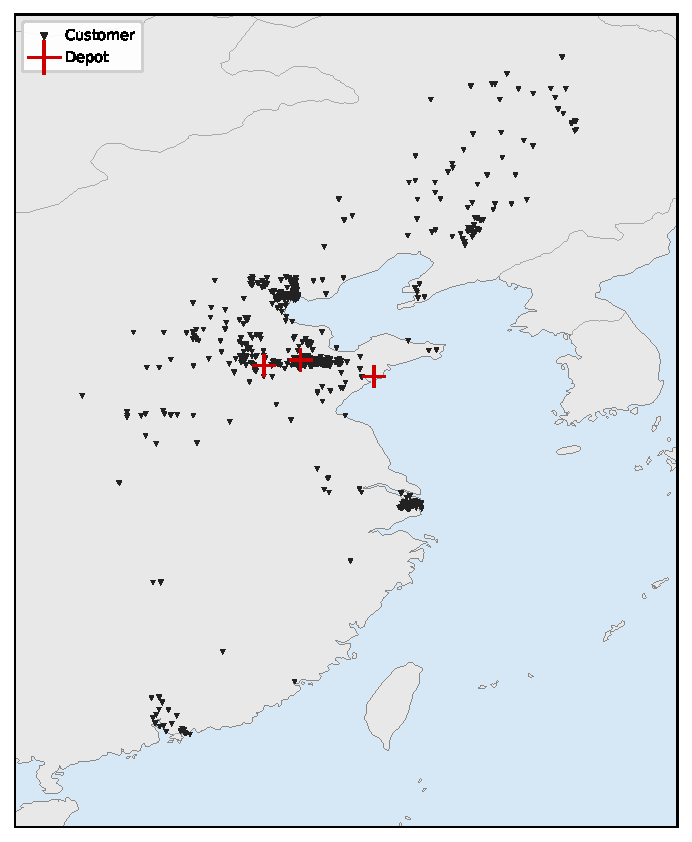
\includegraphics[width=0.55\linewidth]{china_network.pdf}
  \caption{Case study logistics network: eastern coastal China.
           Red crosses = first-echelon depots; triangles = customer locations
           (all 30 planning days overlaid).}
  \label{fig:china_net}
\end{figure}

\begin{table}[H]
\centering
\caption{Optimal Number of Active Satellites per Planning Day (INSGA3)}
\label{tab:satellite}
\small
\begin{tblr}{
    colspec = {c r r r r},
}
\hline[0.08em]
Day & Sat=1 (\$) & Sat=2 (\$) & Sat=3 (\$) & Optimal \\ \hline[0.05em]
 1 &  *4352.4 &  5116.3 &  4596.2 & 1 \\
 2 &  7245.8  & *5490.8 &  6536.2 & 2 \\
 3 &  4704.0  &  4727.1 & *4228.4 & 3 \\
 4 &  5054.9  & *4647.6 &  5727.6 & 2 \\
 5 & *4937.0  &  5847.5 &  5665.1 & 1 \\
 6 &  5995.4  & *5456.1 &  6415.0 & 2 \\
 7 &  5030.5  &  6326.8 & *4788.6 & 3 \\
 8 &  6995.6  &  8352.5 & *6859.7 & 3 \\
 9 & *6748.7  &  7906.2 &  8252.9 & 1 \\
10 &  6067.5  & *5358.8 &  6315.7 & 2 \\
11 & *8451.4  & 10463.6 &  9624.0 & 1 \\
12 &  8473.5  & 10803.7 & *8207.0 & 3 \\
13 &  8411.5  & *7693.6 &  9084.1 & 2 \\
14 &  5924.5  & *5730.8 &  7597.7 & 2 \\
15 &  7236.2  &  8749.8 & *6808.3 & 3 \\
16 & *8937.4  & 10259.9 &  9017.7 & 1 \\
17 & *9047.0  & 10811.8 &  9405.6 & 1 \\
18 &  6864.4  &  6638.3 & *6318.4 & 3 \\
19 &  8658.2  & 10110.7 & *8577.1 & 3 \\
20 &*10992.3  & 14168.2 & 12544.5 & 1 \\
21 &*10224.5  & 13041.5 & 14010.6 & 1 \\
22 & 10421.2  & 11311.9 & *8635.3 & 3 \\
23 &*10859.6  & 12270.4 & 12178.2 & 1 \\
24 & 13091.2  & 14072.8 & *9399.1 & 3 \\
25 &  7793.4  & *6850.4 &  6853.7 & 2 \\
26 & 11020.8  & *9938.2 & 11266.9 & 2 \\
27 &*10860.4  & 13789.6 & 13264.6 & 1 \\
28 & 11257.9  & 12449.2 & *8214.7 & 3 \\
29 &*10319.4  & 12769.5 & 10776.4 & 1 \\
30 &*11258.9  & 12603.7 & 11808.2 & 1 \\
\hline[0.08em]
\SetCell[c=5]{l} \small * denotes minimum cost for that day. \\
\end{tblr}
\end{table}
\noindent\small\textbf{Distribution:} Sat=1: 12 days (40\%), Sat=2: 8 days (27\%), Sat=3: 10 days (33\%).\par\normalsize

The optimal satellite count varies substantially across the 30 days:
Sat=1 is optimal on 40\% of days (12 days), Sat=3 on 33\% (10 days), and
Sat=2 on 27\% (8 days).  This non-monotone distribution confirms that
neither a fixed configuration nor a simple rule of ``more satellites yield
lower cost'' holds across all days; the trade-off between routing savings
and deployment cost is highly sensitive to the daily demand pattern.
Days with larger or more geographically dispersed customer demand tend to
benefit from three satellite depots, whereas days with lighter or more
concentrated demand are served more economically by a single satellite depot.

\Cref{fig:case_trends} reports the day-by-day trends of total cost, vehicle
count (NV), and carbon emissions (CO\textsubscript{2}) across all four satellite
policies.  Activating more satellites generally increases the number of
second-echelon vehicles required to cover the additional intermediate stops;
however, the shorter per-vehicle routes that result can reduce total emissions
when customer demand is spatially dispersed.  Dynamic selection resolves this
trade-off on a daily basis, choosing the configuration that minimises cost while
implicitly adapting NV and emissions to the demand structure of each day.

\begin{figure}[H]
  \centering
  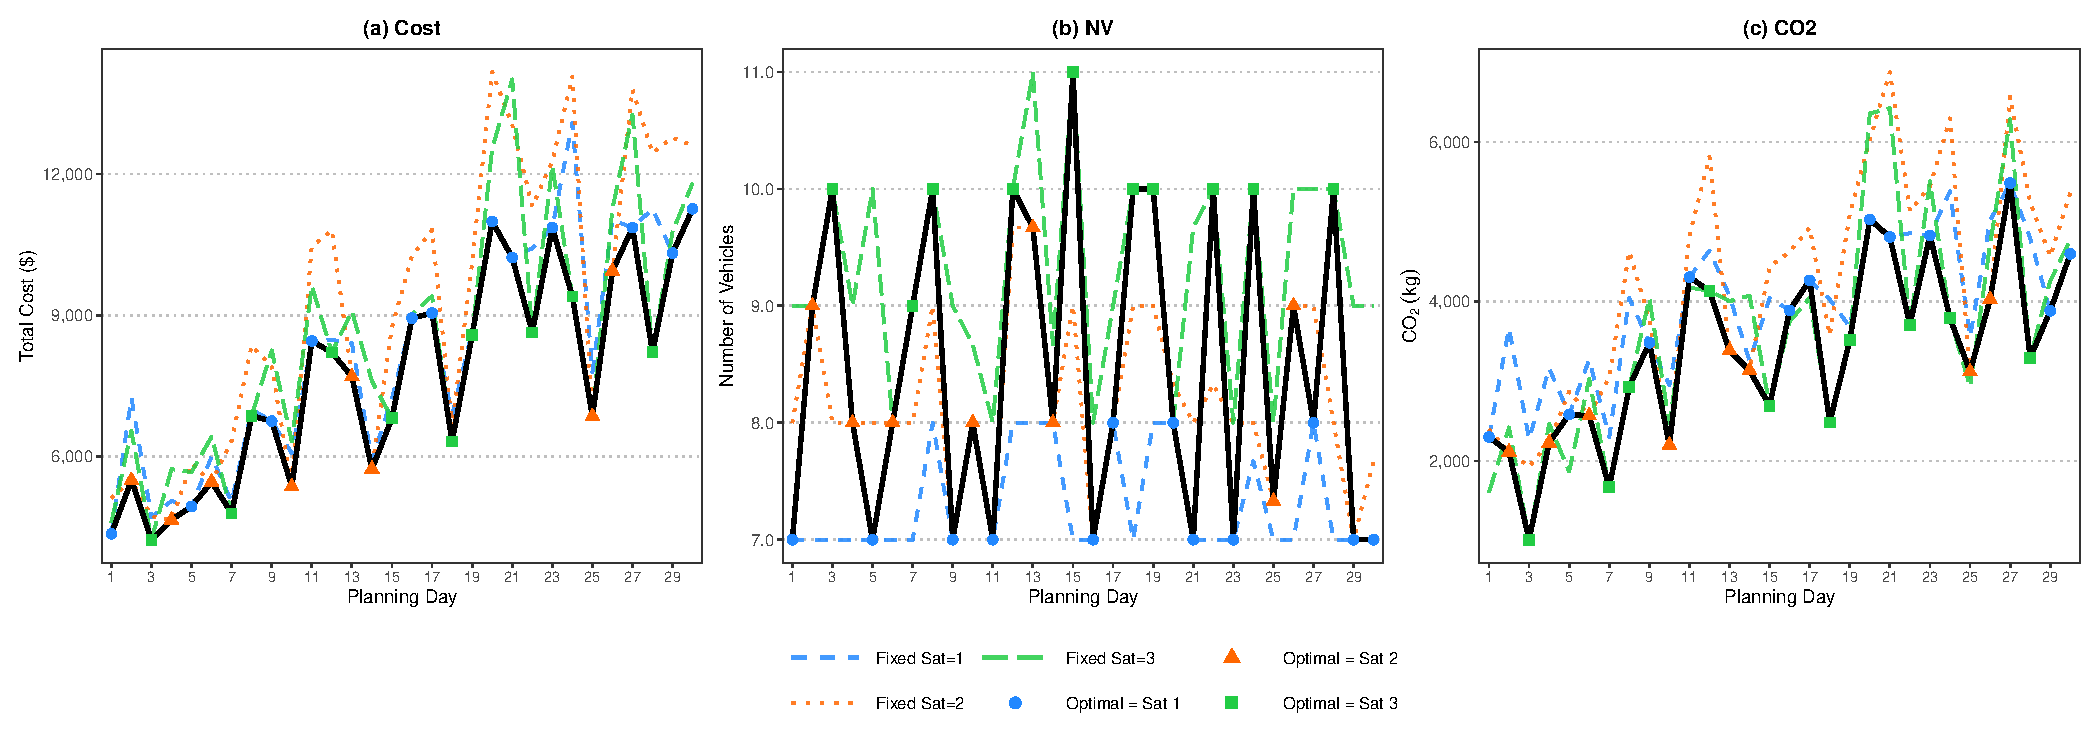
\includegraphics[width=\linewidth]{figures/case_trends_combined_r.pdf}
  \caption{30-day trends under dynamic and fixed satellite configurations:
           (a) total cost---dashed, dotted, and long-dashed lines represent
           Fixed Sat=1, Sat=2, and Sat=3, respectively; the solid black line
           is the dynamic optimal; filled markers (circle/triangle/square)
           indicate the satellite count selected as optimal on each day;
           (b) vehicle count (NV);
           (c) CO\textsubscript{2} emissions.}
  \label{fig:case_trends}
\end{figure}

To quantify the value of dynamic satellite selection across all three
objectives, the 30-day totals for cost, vehicle count (NV), and carbon
emissions (CO\textsubscript{2}) under the dynamic configuration are compared
against three fixed-satellite baselines.  \Cref{tab:dynfixed} summarizes the
results.

\begin{table}[H]
\centering
\caption{30-Day Performance: Dynamic vs.\ Fixed Satellite Policies}
\label{tab:dynfixed}
\small
\begin{tblr}{
    colspec = {l r r r},
}
\hline[0.08em]
Policy & Total Cost (\$) & NV & CO\textsubscript{2} (kg) \\ \hline[0.05em]
Dynamic (optimal per day) & 230{,}192.1 & 254.0 & 101{,}442.7 \\
Fixed Sat=1               & 247{,}235.5 & 219.7 & 118{,}424.5 \\
Fixed Sat=2               & 273{,}757.5 & 246.0 & 126{,}215.4 \\
Fixed Sat=3               & 252{,}977.5 & 279.0 & 108{,}421.9 \\
\hline[0.08em]
\end{tblr}
\end{table}

Dynamic selection achieves the lowest cost and carbon emissions among all
policies.  In terms of cost, it reaches \$230{,}192.1; by comparison, Fixed Sat=1
costs 7.4\% more (\$17{,}043), Fixed Sat=2 costs 18.9\% more (\$43{,}565),
and Fixed Sat=3 costs 9.9\% more (\$22{,}785).  For carbon emissions, the
dynamic policy produces 101{,}442.7\,kg of CO\textsubscript{2}; by comparison,
Fixed Sat=1 produces 16.7\% more (118{,}424.5\,kg), Fixed Sat=2 produces
24.4\% more (126{,}215.4\,kg), and Fixed Sat=3 produces 6.9\% more
(108{,}421.9\,kg).  Although Fixed Sat=1 uses the fewest vehicles (219.7), it incurs higher
emissions because a single satellite forces longer second-echelon routes.
Fixed Sat=3 deploys the most vehicles (279.0) and therefore achieves lower
emissions than Sat=1 and Sat=2, yet still exceeds the dynamic policy in both
cost and CO\textsubscript{2}.  These results show that INSGA3's adaptive satellite
deployment is not merely a cost-minimization heuristic: by selecting the
configuration best suited to each day's demand geography, it simultaneously
reduces routing cost and carbon emissions relative to any rigid
fixed-satellite strategy.

% ============================================================
\section{Conclusion}
\label{sec:conc}
% ============================================================

This section summarizes the contributions of the study, discusses the
limitations of the proposed framework, and outlines promising directions for
future research.

\subsection{Summary of Contributions}

This study addressed the 2E-MD-MD-MP-CVRP-SPD, simultaneously minimizing
total logistics cost ($f_1$), total vehicle count ($f_2$), and total
carbon emissions ($f_3$).  INSGA3 was proposed with a novel triple
initialization strategy over standard NSGA-III: (i)~Logistic Chaos Map
($r=3.9$) for diversity, (ii)~Spatial K-Medoids (PAM) for demand-balanced
cluster seeding, and (iii)~Temporal-Spatial K-Medoids incorporating
time-window midpoints for time-aware ordering.  The evolutionary loop uses
OBX crossover and inversion mutation without any local search.  Carbon
emissions were quantified using the MEET model~\cite{hickman1999}; FE routing
was solved exactly by Gurobi MILP after SE routing was optimized by INSGA3.

Key experimental findings from 20 benchmark instances:
\begin{itemize}
  \item \textbf{Cost}: INSGA3 achieves the lowest average cost
        (\$9{,}575.6 vs.\ \$10{,}562.7 for NSGA-III, a 9.3\% improvement;
        vs.\ \$10{,}643.2 for NSGA-II, a 10.0\% improvement), obtaining
        the best per-instance cost in 18 of 20 instances against NSGA-III
        and 19 of 20 against NSGA-II\@.
  \item \textbf{Pareto front quality}: INSGA3 achieves 10.5\% lower GD
        (0.0214 vs.\ 0.0239) and 9.7\% lower IGD (0.0430 vs.\ 0.0476)
        than NSGA-III, indicating that its solutions are substantially
        closer to and more completely covering the best-known Pareto frontier.
  \item \textbf{Statistical significance}: With $n=10$ runs per instance,
        statistical power is limited; most instances do not reach significance
        under Holm-Bonferroni correction ($m=20$, rank-1 threshold 0.0025).
        The practical advantages of INSGA3 are evidenced by consistent
        cost leadership and substantially better Pareto front quality metrics.
  \item \textbf{Satellite configuration}: The optimal number of active
        satellites varies strongly by day (Sat=1: 40\%, Sat=2: 27\%,
        Sat=3: 33\%), demonstrating the necessity of the multi-period
        formulation.
\end{itemize}

\subsection{Managerial Implications}

The proposed framework offers several practical insights for logistics operators
and supply chain managers.  First, INSGA3's triple initialization produces
high-quality diverse starting populations, yielding solutions that are
consistently closer to the Pareto optimum (GD improvement: 10.5\%) without
the computational overhead of embedded local search; managers benefit from
competitive solver runtimes (avg 71.4\,s) and superior solution quality.  Second, the satellite configuration case study
demonstrates that the cost-optimal number of active satellites varies
substantially across days (Sat\,=\,1: 40\%, Sat\,=\,2: 27\%, Sat\,=\,3:
33\%); dynamic deployment achieves cost reductions of 7.4\%--18.9\% and
CO$_2$ reductions of 6.9\%--24.4\% relative to any fixed-satellite policy
over the 30-day horizon.  Managers should therefore adopt demand-driven
dynamic satellite deployment rather than a fixed configuration.  Third, the MEET-based carbon
objective enables simultaneous tracking of cost and carbon footprint, directly
supporting ESG reporting and compliance with tightening emission regulations.
Fourth, the two-echelon decomposition---INSGA3 for second-echelon routing
and Gurobi MILP for first-echelon assignment---provides a scalable
decision-support tool for large logistics networks with multiple depots and
satellite facilities.  Finally, the simultaneous pickup and delivery formulation
allows return collection on outbound routes, reducing empty return trips and
lowering total vehicle deployment.

\subsection{Limitations}

(1)~Soft time windows; hard-window extension would require additional
feasibility repair mechanisms.  (2)~The real-world case study is limited to a single geographic region;
broader cross-region validation remains an important future step.  (3)~Sequential FE-SE
decomposition may yield suboptimal solutions relative to joint optimization
in some cases.  (4)~Homogeneous fleet assumption; heterogeneous or electric
vehicles are not modeled.  (5)~Sample size $n=10$ limits statistical power;
larger sample sizes are needed to draw more definitive statistical conclusions.
(6)~Broader baseline comparison with other established MOEAs applied to
2E-VRP variants would further contextualize INSGA3's competitiveness.  (7)~An ablation study isolating the marginal contribution
of each initialization method (Chaos Map, Spatial K-Medoids,
Temporal-Spatial K-Medoids) remains outstanding.

\subsection{Future Research Directions}

(1)~Hard time-window extension with feasibility-aware decoding.
(2)~Real-world validation on empirical logistics datasets.
(3)~Joint FE-SE co-evolutionary or bi-level optimization.
(4)~Green vehicle integration (electric fleets, range constraints, charging
schedules).
(5)~Dynamic/stochastic demand via robust or stochastic optimization.
(6)~Systematic ablation study quantifying the marginal contribution of each
INSGA3 initialization component (Chaos Map, Spatial K-Medoids,
Temporal-Spatial K-Medoids) and broader comparative evaluation with
additional MOEA baselines beyond those tested.
(7)~Increasing the per-instance run count to $n\ge30$ and reporting effect
sizes (rank-biserial correlation) and 95\% bootstrap confidence intervals to
support stronger statistical conclusions.
(8)~Investigation of adaptive parameter control for $cp$, $mp$, and the
logistic map parameter~$r$ to further improve INSGA3 robustness across
diverse instance structures.

% ============================================================
\printbibliography
% ============================================================

\end{document}
